%% IFBThesis Latex Template Version 1.0, a fork of :
%% 	RiSE Latex Template - version 0.5
%%
%% IFBthesis latex template for thesis and dissertations
%% https://github.com/auyer/IFBtcc
%%
%% (c) 2017 Rafael de Campos Passos (rcpassos@ieee.org)
%%
%% This document was initially based on RiSE Latex template, from Yguaratã
%% Cerqueira Cavalcanti
%%
%% GENERAL INSTRUCTIONS
%%
%% We strongly recommend you to compile your documents using pdflatex command.
%% It is also recommend use the texlipse plugin for Eclipse to edit your documents.
%%
%% Options for \documentclass command:
%%         * Idiom
%%           pt   - Portguese (default)
%%           en   - English
%%
%%         * Text type
%%           bsc  - B.Sc. Thesis
%%           msc  - M.Sc. Thesis (default)
%%           qual - PHD qualification (not tested yet)
%%           prop - PHD proposal (not tested yet)
%%           phd  - PHD thesis
%%
%%         * Media
%%           scr  - to eletronic version (PDF) / see the users guide
%%
%%         * Pagination
%%           oneside - unique face press
%%           twoside - two faces press
%%
%%		   * Line spacing
%%           singlespacing  - the same as using \linespread{1}
%%           onehalfspacing - the same as using \linespread{1.3}
%%           doublespacing  - the same as using \linespread{1.6}
%%
%% Reference commands. Use the following commands to make references in your
%% text:
%%          \figref  -- for Figure reference
%%          \tabref  -- for Table reference
%%          \eqnref  -- for equation reference
%%          \chapref -- for chapter reference
%%          \secref  -- for section reference
%%          \appref  -- for appendix reference
%%          \axiref  -- for axiom reference
%%          \conjref -- for conjecture reference
%%          \defref  -- for definition reference
%%          \lemref  -- for lemma reference
%%          \theoref -- for theorem reference
%%          \corref  -- for corollary reference
%%          \propref -- for proprosition reference
%%          \pgref   -- for page reference
%%
%%          Example: See \chapref{chap:introduction}. It will produce
%%                   'See Chapter 1', in case of English language.
%%
%% Citation commands:
%%          \citet (from natbib) -- To cite a reference as part of the narrative
%%          \citep (from natbib) -- To cite a reference between parenthesis
%%          citationblock environment -- To produce direct citation blocks according to the ABNT

\documentclass[pt,twoside,onehalfspacing,bsc]{ifgtcc}


\usepackage{colortbl}
\usepackage{color}
\usepackage[table]{xcolor}
\usepackage{microtype}
\usepackage{bibentry}
\usepackage{subfigure}
\usepackage{multirow}
\usepackage{rotating}
\usepackage{booktabs}
\usepackage{pdfpages}
\usepackage{caption}
\usepackage{lipsum}
\usepackage{sectsty}
%pages
\usepackage{lastpage}
\usepackage{float}

%% Set the language used in your code in the block above

\captionsetup[table]{position=top,justification=centering,width=.85\textwidth,labelfont=bf,font=footnotesize}
\captionsetup[lstlisting]{position=top,justification=centering,width=.85\textwidth,labelfont=bf,font=footnotesize}
\captionsetup[figure]{position=bottom,justification=centering,width=.85\textwidth,labelfont=bf,font=footnotesize}

%% Chapter and (Sub)Section fonts must be same size as text (12)
\sectionfont{\fontsize{12}{15}\selectfont}
\subsectionfont{\fontsize{12}{15}\selectfont}
\subsubsectionfont{\fontsize{12}{15}\selectfont}

%% Change the following pdf author attribute name to your name.
\usepackage[linkcolor=black,
            citecolor=black,
            urlcolor=black,
            colorlinks,
            pdfpagelabels,
            pdftitle={Rise Thesis Template (ABNT)},
            pdfauthor={Rise Thesis Template (ABNT)},
            breaklinks=true]{hyperref}

\address{FORMOSA}

\universitypt{Instituto Federal de Goiás}
\universityen{Federal Institute of Goi\'as}

\campus{{\it Campus} Formosa}

\departmentpt{Departamento de Áreas Acadêmicas}
\departmenten{Academic Department}

\programpt{Análise e Desenvolvimento de Sistemas}
\programen{Systems Analyses and Develpment}

\majorfieldpt{Ciência da Computação}
\majorfielden{Computer Science}

\title{{\emph e-Plano}: Plano Semestral de Trabalho Docente}

\date{2019}

\author{Maryana Marinho da Silva Melo}
\adviser{Prof. Dr. Waldeyr Mendes Cordeiro da Silva}
%\coadviser{Nome dompleto do co-orientador }

% Macros (defines your own macros here, if needed)
\def\x{\checkmark}
%\let\lstlistoflistings\origlstoflistings
\begin{document}

\frontmatter

\frontpage

\presentationpage

\begin{fichacatalografica}
\FakeFichaCatalografica % Comment this line when you have the correct file
%\includepdf{fig_ficha_catalografica.pdf} % Uncomment this
\end{fichacatalografica}


%NAO APAGAR ISSO AQUI
%\banca

\begin{ata}
\begin{figure}
	\centering 
	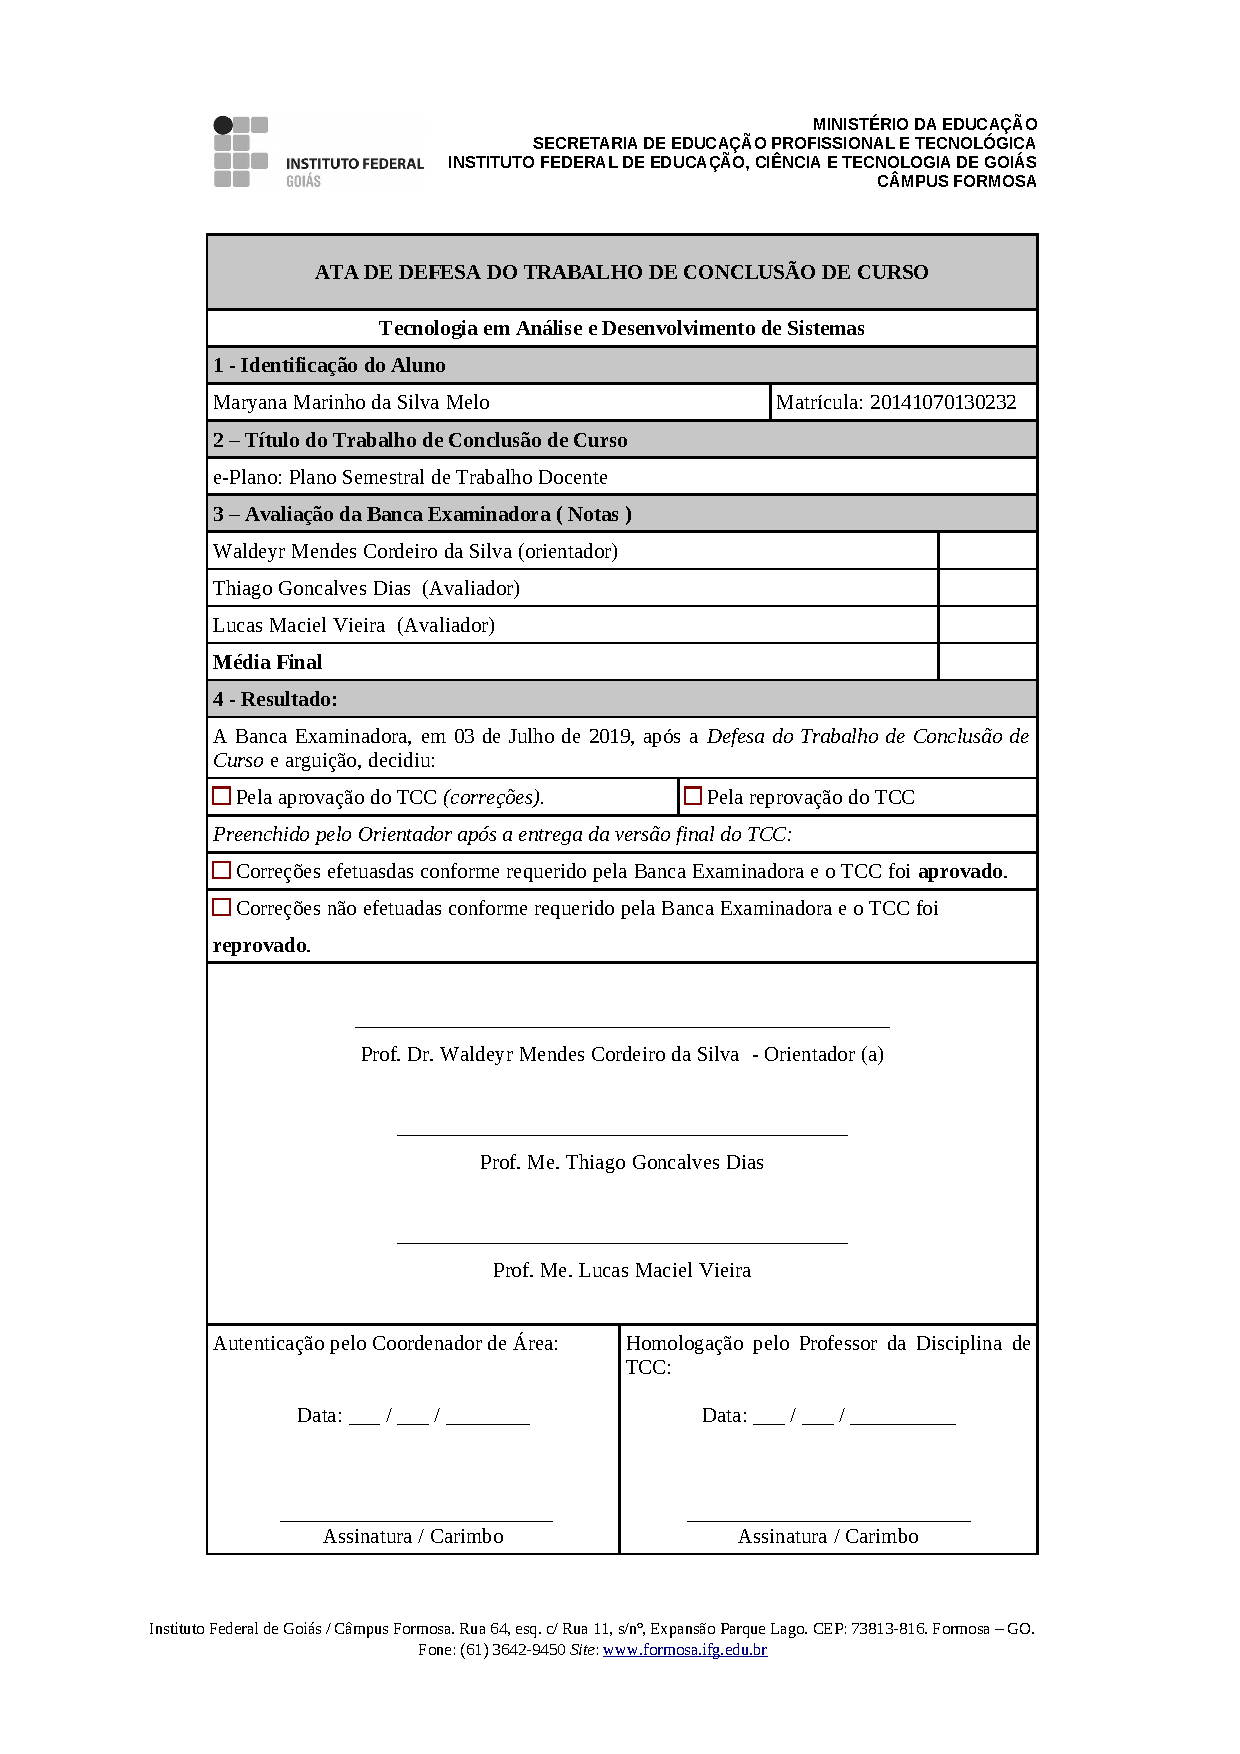
\includepdf[pages=-,width=\textwidth]{doc/Ata.pdf}
\end{figure}
\end{ata}


\begin{ata}
	\begin{figure}
		\centering 
		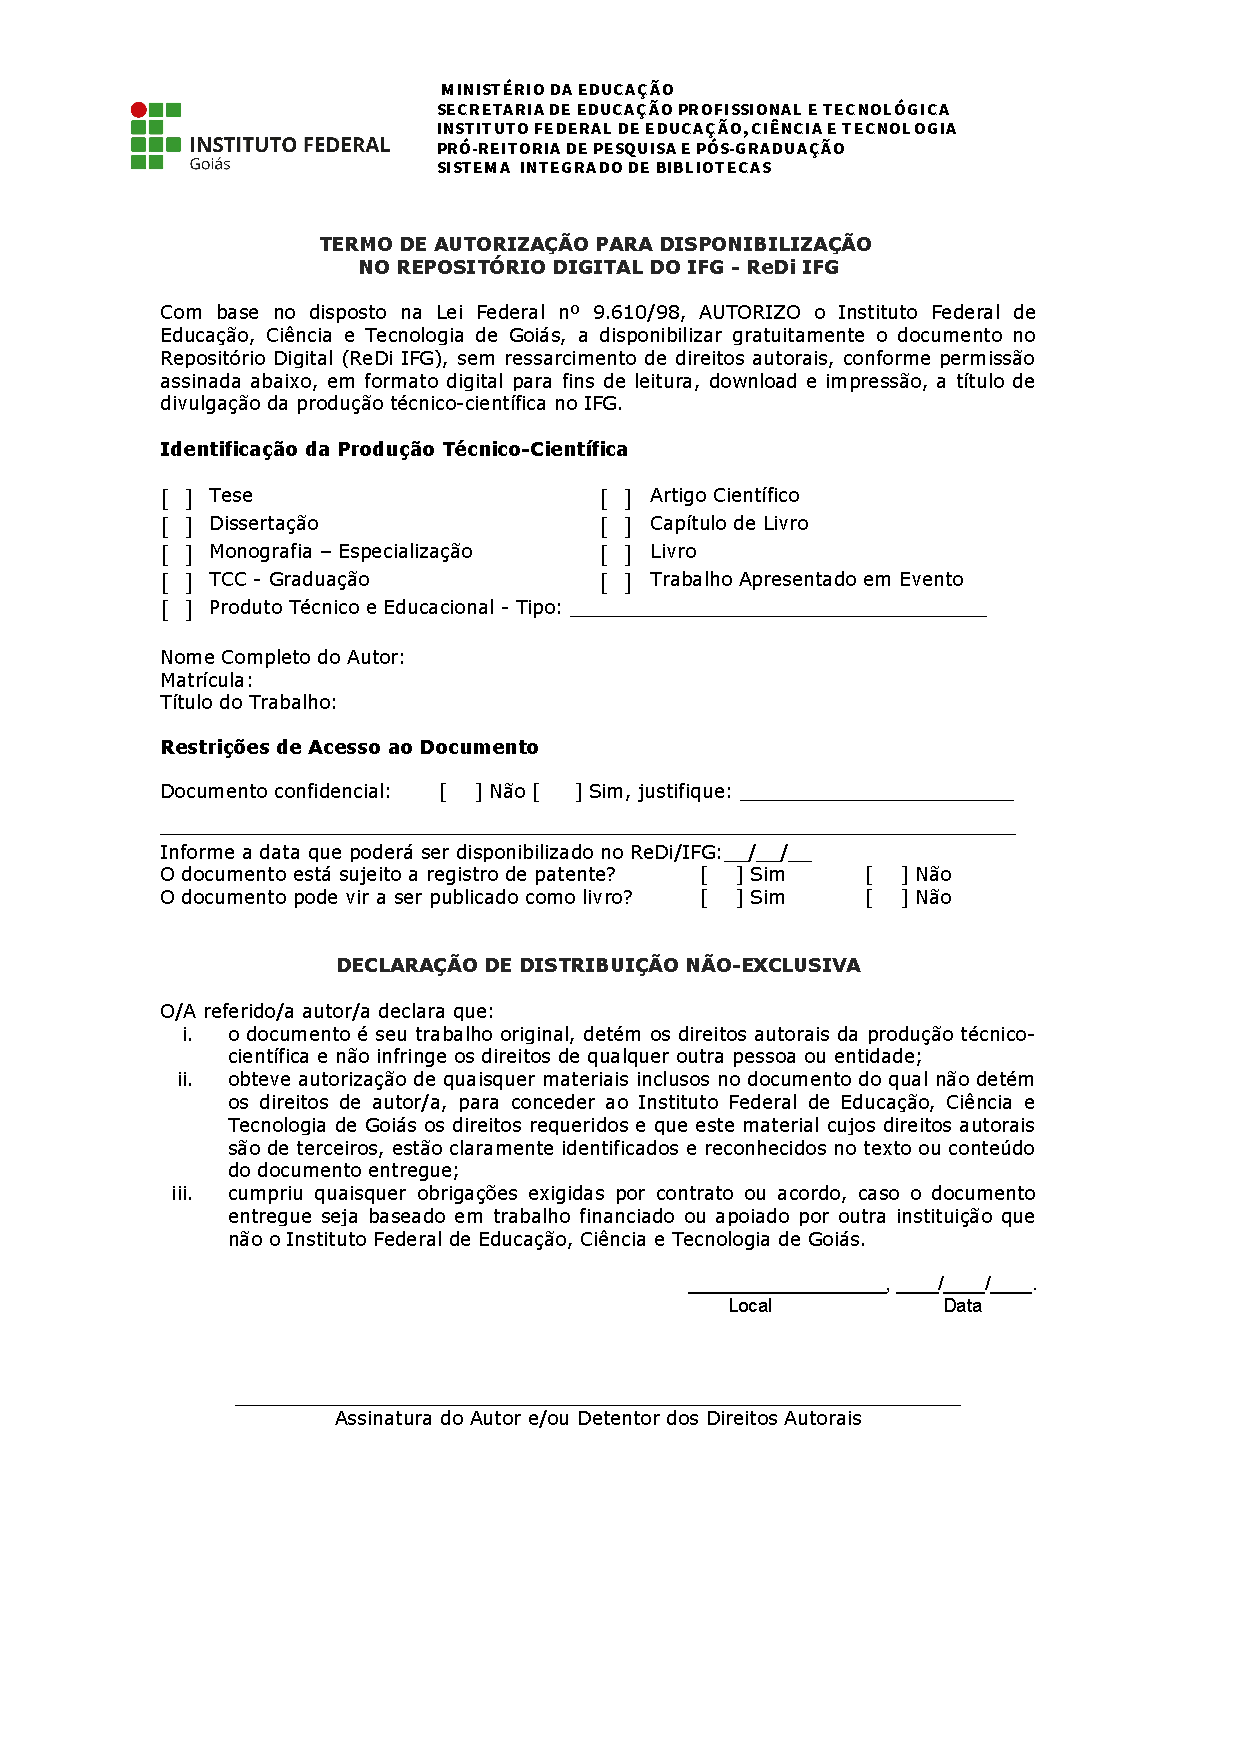
\includepdf[pages=-,width=\textwidth]{doc/redi.pdf}
	\end{figure}
\end{ata}



\begin{dedicatory}
Eu dedico este trabalho a todas as meninas e mulheres que sonham em trabalhar com ciência ou tecnologia. 
\end{dedicatory}

% \acknowledgements
% \lipsum[1-4]

Agradeço a minha mãe por me apoiar sempre, e por fazer eu chegar ate aqui. Sem ela não seria possível.
Ao meu orientador professor Dr. Waldeyr Mendes Cordeiro da Silva, pelo conhecimento, orientação e compreensão.
Aos meus amigos pelo apoio, incentivo e torcida pelo meu sucesso.
A todos que me ajudaram direta ou indiretamente nessa nessa jornada. 


% \begin{epigraph}[]{Márcio de Deus}
% When one finds a hard problem, the more complicated it is, the more one ought to work towards enlightening it's solution.
% \end{epigraph}

\resumo
% Escreva seu resumo no arquivo resumo.tex
{\parindent0pt
	O \acf{IFG} é uma instituição pública que oferta cursos de educação básica, profissional e superior. 
Os docentes do \ac{IFG} precisam apresentar semestralmente o ``Plano Semestral de Trabalho Docente'' com o planejamento das atividades a serem realizadas e suas respectivas cargas horárias e pontuações de acordo com a Resolução 09 de 1º de Novembro de 2011.
Todos os dados são convertidas em pontos de acordo com fatores de ponderação, sendo um instrumento de planejamento tanto do docente quanto do \acf{DAA} do \ac{IFG}. 
Entretanto, os planos de trabalho semestrais são baseados em modelos de documentos de texto e planilha eletrônica.
Esse cenário é propício para problemas de preenchimento que levam frequentemente a planos de trabalho em desacordo com a norma.
Utilizando tecnologias atuais de mercado foi desenvolvida uma aplicação \textit{web} chamada ``\textit{e}-Plano''.
O \textit{e}-Plano foi desenvolvido para funcionar de forma independente de sistema operacional, responsivo ao tamanho da tela no \textit{browser} e com interface amigável ao usuário.
Tais características foram fruto da aplicação de diversas técnicas e metodologias de desenvolvimento de software, com vistas a facilitar o preenchimento do ``Plano Semestral de Trabalho Docente'' garantindo sua conformidade com a Resolução 09 de 1º de Novembro de 2011.

\begin{keywords}
Plano Semestral de Trabalho Docente, IFG, desenvolvimento de software, aplicação \textit{Web} 
\end{keywords}
}

\abstract
% Write your abstract in a file called abstract.tex
{\parindent0pt
	IFG is a public institution offering primary, professional, and higher education courses.
The teachers of the IFG must present the "Semester Work Plan" semiannually with the planning of the activities to be carried out and their respective schedules according to Resolution number 09, of November 01, 2011.
This resolution preconizes that all data are converted into points weighting factor, being a planning tool both for the teacher and the \acf{DAA} of \ac{IFG}.
However, there is no system to consolidate such a resource, which is currently done using papers based on a sheet and text document models.
A web application called ``{\it e-Plan}'' was developed to address this problem and give a digital solution.
\textit{e}-Plano has been designed to work independently of the operating system, responsive to screen size in the browser and with a user-friendly interface.
These characteristics were achieved by the employment of several software development techniques and methodologies.
The result is a Web application that facilitates the fulfillment of the document ensuring compliance of the "Semester Work Plan" with Resolution 09, from November 01, 2011.

\begin{keywords}
Semester Work Plan, IFG, software development, \textit{Web} application
\end{keywords}
}

% List of figures
\listoffigures

% List of Codes
%\lstlistoflistings

% List of tables
\listoftables

% List of acronyms
% Acronyms manual: http://linorg.usp.br/CTAN/macros/latex/contrib/acronym/acronym.pdf
\listofacronyms
\begin{acronym}[ACRONYM] 
% Não é necessário ordenar as siglas
\acro{IFG}[IFG]{Instituto Federal de Educação, Ciência e Tecnologia de Goiás}
\acro{DAA}[DAA]{Departamento de Áreas Acadêmicas}
\acro{Cefet}[Cefet]{Centros Federais de Educação Profissional e Tecnológica}
\acro{Uneds}[Uneds]{Unidade de Ensino Descentralizada}
\acro{ETFG}[ETFG]{Escola Técnica Federal de Goiás}
\acro{URL}[URL]{Uniform Resource Locator}
\acro{HTML}[HTML]{Hypertext Markup Language}
\acro{CSS}[CSS]{Cascading Style Sheets}
\acro{SGBDs}[SGBDs]{Sistema de Gerenciamento de Banco de Dados}
\acro{SQL}[SQL]{Structured Query Language}
\acro{NoSQL}[NoSQL]{Not Only SQL}
\acro{REST}[REST]{Representational State Transfer}
\acro{HTTP}[HTTP]{Hypertext Transfer Protocol}
\acro{URI}[URI]{Uniform Resource Identifier}
\acro{JSON}[JSON]{JavaScript Object Notation}
\acro{PDF}[PDF]{Portable Document Format}
%%
\acro{afm}[AFM]{Alphabet Frequency Matrix}
\acro{api}[API]{Application Programming Interface}
\acro{arima}[ARIMA]{Auto-Regressive Integrated Moving Average}
\acro{brn}[BRN]{Bug Report Network}
\acro{bts}[BTS]{Bug Triage System}
\acro{cas}[CAS]{Context-Aware Systems}
\acro{ccb}[CCB]{Change Control Board}
\acro{cr}[CR]{Change Request}
\acro{cvs}[CVS]{Concurrent Version System}
\acro{es}[ES]{Expert System}
\acro{floss}[FLOSS]{Free/Libre Open Source Software}
\acro{glr}[GLR]{Generalized Linear Regression}
\acro{gqm}[GQM]{Goal Question Metric}
\acro{html}[HTML]{HyperText Markup Language}
\acro{ir}[IR]{Information Retrieval}
\acro{irt}[IRT]{Recôncavo Institute of Technology}
\acro{jdt}[JDT]{Jazz Duplicate Finder}
\acro{lda}[LDA]{Latent Dirichlet Allocation}
\acro{loc}[LOC]{Lines of Code}
\acro{lsi}[LSI]{Latent Semantic Indexing}
\acro{ms}[MS]{Mapping Study}
\acro{msr}[MSR]{Mining Software Repositories}
\acro{nlp}[NLP]{Natural Language Processing}
\acro{promise}[PROMISE]{Predictive Models in Software Engineering}
\acro{rbes}[RBES]{Rule-Based Expert System}
\acro{rhel}[RHEL]{RedHat Enterprise Linux}
\acro{saas}[SaaS]{Software as a Service}
\acro{scm}[SCM]{Software Configuration Management}
\acro{serpro}[SERPRO]{Brazilian Federal Organization for Data Processing}
\acro{slr}[SLR]{Stepwise Linear Regression}
\acro{slr}[SLR]{Systematic Literature Review}
\acro{svd}[SVD]{Singular Value Decomposition}
\acro{svm}[SVM]{Support Vector Machine}
\acro{svn}[SVN]{Subversion}
\acro{tfidf}[TF-IDF]{Term Frequency-Inverse Document Frequency}
\acro{vsm}[VSM]{Vector Space Model}
\acro{xp}[XP]{Extreming Programming}
\acro{gui}[GUI]{Graphical User Interface}
\end{acronym}

% Summary (tables of contents)
\tableofcontents

\mainmatter

\chapter{Introdução}
\label{chp:introducao}

Em Dezembro de 2008, através da Lei nº 11.892, de 29 de Dezembro de 2008, foram criados os  Institutos Federais de Educação, Ciência e Tecnologia, que são instituições de educação superior, básica e profissional, pluricurriculares e \textit{multicampi}, especializados em oferecer educação profissional e tecnológica nas variadas formas de ensino, e equiparadas as universidades federais~\citep{lei11892}.

Os Institutos Federais estão espalhadas por todo o território brasileiro, havendo no mínimo mais de um instituto por estado, qualificando profissionais para os inúmeros setores da economia, realizando pesquisa e desenvolvendo novos processos, produtos e serviços~\citep{historiaif}. 

O \acf{IFG}, atualmente tem reitoria, sede e foro na cidade de Goiânia e possui 14 câmpus.
Entretanto, a história do IFG precede sua atual organização administrativa tendo nascido como Escolas de Aprendizes Artífices em 1909, que na época tinha o objetivo de capacitar os alunos em cursos e oficinas de forjas e serralheria, sapataria, alfaiataria, marcenaria e empalhação, selaria e correaria. 
Em 1942 virou Escola Técnica de Goiânia e teve a criação de cursos técnicos na área industrial, integrados ao ensino médio, por meio do Decreto-lei n.º 4.127, de 25 de fevereiro de 1942. 
Já em 1959 adquiriu a condição de autarquia federal e em 1965 tornou-se Escola Técnica federal de Goiás (ETFG)~\citep{historiaifg}. 
Em 1999 se tornou Centro Federal de Educação Tecnológica de Goiás (CEFET-GO), com autorização para ofertar cursos superiores, que no início tinha como política ser voltado para as "classes desprovidas", sendo uma instituição pública e gratuita. Para enfim em Dezembro de 2008, se transformar em Instituto Federal de Educação, Ciência e Tecnologia~\citep{historiaif}. 

Em sua organização administrativa atual, o IFG possui instâncias colegiadas, comissões, comitês e fóruns permanentes, reitoria, e os \textit{campi}. 
Incluída essas organizações administrativas, está a comunidade acadêmica, que é composta pelo corpo discente, docente e técnico-administrativo~\citep{regimentoifg}.
O corpo docente é composto pelos professores do quadro de pessoal definitivo do IFG, gerenciados pelo Regime Jurídico Único~\citep{brasil1990lei}, e demais professores admitidos na forma da legislação em vigor~\citep{regimentoifg}.

Nos \textit{campi}, os Departamentos de Áreas Acadêmicas (DAA) programam as atividades acadêmicas a serem desenvolvidas pelos servidores docentes, e distribuem a carga horária semanal de trabalho de acordo com o seu regime de trabalho, que podem ser de 20 horas semanais, 40 horas semanais, ou 40 horas semanais com dedicação exclusiva~\citep{resolucao}.

De acordo com Resolução 09 de 1º de Novembro de 2011, as atividades acadêmicas dos docentes são convertidas em pontos, e a somatória desses pontos devem totalizar a carga horária do regime de trabalho do servidor~\citep{resolucao}.
As atividades realizadas pelos docente compreendem ensino, pesquisa e extensão, e por isso diversos critérios foram criados nesta resolução para estabelecer a correlação entre as diversas atividades e a carga horária~\citep{resolucao}.

Obedecendo à Resolução 09 de 1º de Novembro de 2011~\citep{resolucao}, os docentes precisam apresentar um Plano Semestral de Trabalho e ao fim do semestre um Relatório Semestral de Trabalho.
O Plano Semestral de Trabalho tem sido preenchido através de um modelo em um documento no Microsoft Word$^{\circledR}$, e fazem suas somatórias de pontos em uma planilha Microsoft Excel$^{\circledR}$. 
Esse procedimento é propenso a problemas como diferentes formas de preenchimento de acordo com o entendimento do docente, não conformidade nas somas de pontos e falta de clareza em documento oficial.
Diante do exposto, este trabalho propõe uma solução para o docente preencher seu Plano de Trabalho Semestral. 
Tal solução tem duas principais características: uma interface amigável ao usuário e a garantia do respeito às normas da Resolução 09 de 1º de Novembro de 2011.

\section{Objetivo}
\indent

Construir uma solução \textit{user-friendly} e independente de sistema operacional para a elaboração do Plano Semestral de Trabalho nos termos da Resolução 09 de 1º de Novembro de 2011 do IFG.

\subsection*{Objetivos Específicos}

\begin{enumerate}
	\item Fazer a prototipação e documentação do sistema a partir do levantamento de requisitos.
	\item Aprovar o protótipo e desenvolver o sistema como uma aplicação web em conformidade com a resolução 09 de 1º de Novembro de 2011~\citep{resolucao}.
	\item Disponibilizar o sistema de forma pública para uso do IFG.
\end{enumerate}




\chapter{Referencial Teórico}
\label{Referencial_Teorico}


\newcommand{\texCommand}[1]{\texttt{\textbackslash{#1}}}%

\newcommand{\exemplo}[1]{%
\vspace{\baselineskip}%
\noindent\fbox{\begin{minipage}{\textwidth}#1\end{minipage}}%
\\\vspace{\baselineskip}}%

\newcommand{\exemploVerbatim}[1]{%
\vspace{\baselineskip}%
\noindent\fbox{\begin{minipage}{\textwidth}%
#1\end{minipage}}%
\\\vspace{\baselineskip}}%


%%%%%%%%%%%%%%%%%%%%%%%%%%%%%%%%%%%%%%%%%%%%%%%%%%%%%%%%%%%%%%%%%%%%%%%%%%%%%%%%
%%%%%%%%%%%%%%%%%%%%%%%%%%%%%%%%%%%%%%%%%%%%%%%%%%%%%%%%%%%%%%%%%%%%%%%%%%%%%%%%
%%%%%%%%%%%%%%%%%%%%%%%%%%%%%%%%%%%%%%%%%%%%%%%%%%%%%%%%%%%%%%%%%%%%%%%%%%%%%%%%
Este capítulo traz informações sobre metodologias, técnicas e ferramentas computacionais que serão usadas para alcançar os objetivos propostos.
A Seção~\nameref{prototipacao} traz uma breve explicação sobre a metodologia de desenvolvimento de software escolhida.
Na Seção~\nameref{TecDesSof} são explorados os conceitos das tecnologias e ferramentas computacionais empregadas neste trabalho.
A Seção~\nameref{GerProj} descreve o gerenciamento de projetos de análise e desenvolvimento de software abordando algumas diferentes e essenciais etapas como o Levantamento de Requisitos, a Validação e a Implantação.

\section{Prototipação}\label{prototipacao}
\indent

A Prototipação é uma metodologia de desenvolvimento de software cuja principal característica é exibir um protótipo do sistema para o cliente antes de sua implementação~\citep{buchenau2000experience}.
É uma abordagem onde tanto o cliente como o desenvolvedor são beneficiados, uma vez que o cliente pode ter acesso a uma interface prévia do sistema, manifestar sua opinião e discutir funcionalidades desejadas, enquanto o desenvolvedor identifica melhor os requisitos e tem uma maior noção do esforço que será delegado no desenvolvimento~\citep{pressmanengenharia}. 
Usando a prototipação, o processo de software funciona como um ciclo de reuniões entre o cliente e o desenvolvedor e interações com o protótipo ate que haja consenso em uma versão final, conforme exemplificado na Figura~\ref{fig:protPressman}.  

\begin{figure}[htbp]
    \centering
    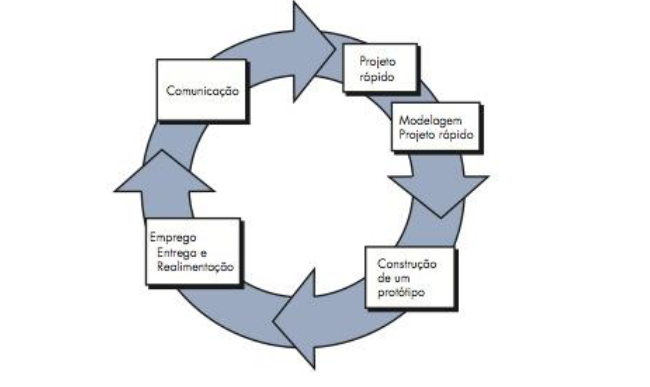
\includegraphics[width=0.75\textwidth]{img/paradigma_prototipacao_pressman.PNG}
    \caption[Paradigma da prototipação]{Paradigma da prototipação. Fonte:~\cite{pressmanengenharia}.}
    \label{fig:protPressman}
\end{figure}

\newpage
\section{Tecnologias de Desenvolvimento de Software}\label{TecDesSof}
\indent

\subsection{\textit{Web}}
\indent

Aplicações \textit{Web} são sistemas cliente/servidor que são acessadas através de um endereço do tipo~\acf{URL} pelo navegador (cliente) que fazem requisições para o servidor~\citep{gonccalves2007}. 
A aplicação pode ser acessada de qualquer dispositivo que tenha internet, independente de \textit{hardware} ou sistema operacionais como Microsoft Windows$^{\circledR}$, Linux diversos, Android, iOS e outros. 

O usuário interage com a aplicação por meio de uma interface processada no navegador e realiza chamadas para o servidor onde está alocada a camada do servidor responsável pelo armazenamento dos dados em conjunto com o banco de dados, e o processamento das regras de negócio~\citep{pereira2018desenvolvimento}.

\subsection{Java}\label{java}
\indent

Java é uma linguagem de programação orientada a objetos, portável, robusta e segura que permite o desenvolvimento de sistemas para a \textit{Web}, \textit{Desktop}, e aparelhos celulares~\citep{mendes2009programaccao}.
Foi criada por James Gosling da Sun Microsystems em 1991, o que chamou atenção na época pois a linguagem podia ser portável para outros sistemas operacionais. Atualmente é utilizada por grandes bancos por ser uma linguagem segura que desfruta de um ecossistema grande e maduro, com forte suporte a ferramentas~\citep{gonccalves2007}. Atualmente o java está na versão 12.0.1
O java possui uma maquina virtual que é conhecida como JVM, ela fornece especificações de \textit{hardware} que permite o java ser uma plataforma independente pois a compilação é feita pela JVM~\citep{mendes2009programaccao}.

\subsection{\textit{Spring Boot}}\label{spring}
\indent

\textit{Spring Boot} é um \textit{framework} criado para agilizar o desenvolvimento de aplicações java pois as configurações necessárias que o desenvolvedor precisa fazer ao iniciar o desenvolvimento de uma aplicação web já vem pre estabelecida, com isso o programador só precisa se preocupar com as regras de negócio~\citep{springboot}.

\subsection{REST}\label{rest}
\indent

\acf{REST} é um modelo de arquitetura para criação de aplicações web que utiliza o protocolo \acf{HTTP} na criação de serviços web com resposta em formato XML ou JSON. 
Uma aplicação é dita RESTful, quando é construída com os princípios básicos do REST~\citep{lecheta2015web}.
O REST tem um conjunto de métodos para a realização das requisições:

\begin{itemize}
    \item \textit{GET} que é utilizado para consulta de dado.
    \item \textit{POST} que é utilizado para inserir dado.
    \item \textit{PUT} que é utilizado para atualização de dado.
    \item \textit{DELETE} que é utilizado para a exclusão de dado.
\end{itemize}

\subsection{Banco de dados}\label{bd}
\indent

Um banco de dados é uma coleção de dados inter-relacionados com a finalidade de fornecer ao usuário o armazenamento dos dados e uma visão abstrata dos dados recuperando-os de maneira eficiente, acessível por sistemas dos mais variados tipos.
O gerenciamento do banco de dados para operações de busca, inserção, atualização e exclusão podem ser realizados por meio de um tipo de software conhecido como \acf{SGBDs}~\citep{silberschatz2016sistema}. 

Existem várias formas de modelar os dados, tais como, o modelo relacional, modelo de entidade/relacionamento, modelo de dados baseado em objeto, modelo de dados semiestruturado entre outros. 
O banco de dados relacional utiliza o modelo relacional que representa os dados e o relacionamento entre eles através de um conjunto de tabelas~\citep{silberschatz2016sistema}.
A linguagem de manipulação dos bancos de dados relacionais é o \acf{SQL}~\citep{silberschatz2016sistema}.

\subsection{MongoDB}\label{mongo}
\indent

Com a utilização em larga escala da \textit{Internet} e com surgimento das redes sociais, o volume de dados vem crescendo rápido.
Com esse crescimento, surgiu a necessidade de manipular e processar grandes quantidades de dados não estruturados, e como solução foi criados os bancos de dados não relacionais ou \acf{NoSQL}. 
O \ac{NoSQL} é um banco não estruturado, flexível com capacidade de escalonamento~\citep{santana2019nosql}. 
Existem vários modelos de dados \ac{NoSQL}, os principais são: Chave-valor, orientado a documentos, orientado a colunas e orientado a grafos~\citep{santana2019nosql}.

MongoDB é um banco de dados não relacional orientada a documento e \textit{open source}, sua representação é simplesmente um conjunto de chave e valor, que permite modificações no documento como adição de novos campos tornando-o flexível e de fácil escalonamento. Os documentos no MongoDB podem ter o tamanho máximo de 16 MB, e utiliza o \acf{JSON} para retornar os resultados das consultas e representar os dados, mas internamente codifica o \ac{JSON} para o \textit{Binary} JSON (BSON). Sua implementação é leve, rápida e eficiente~\citep{mongodb}.
Na Figura~\ref{fig:shell-mongo} é um exemplo de inserção e consulta no \textit{Shell} do MongoDB.

\begin{figure}[H]
    \centering
    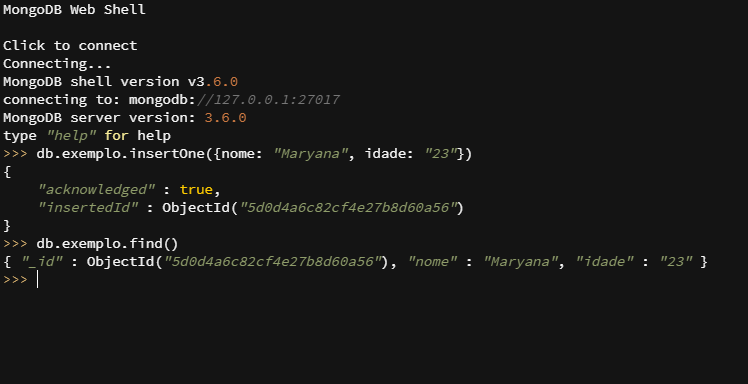
\includegraphics[width=0.95\textwidth]{img/codigo_mongo.PNG}
    \caption[Exemplo no \textit{Shell} do MongoDB]{Exemplo no \textit{Shell} do MongoDB.}
    \label{fig:shell-mongo}
\end{figure}

\subsection{Angular}\label{angular}
\indent

O Angular é um \textit{framework} JavaScript \textit{open source} utilizado na fabricação do \textit{front-end} da aplicação que pode ser tanto web quanto mobile. 
Desenvolvida pela Google, atualmente é um dos \textit{frameworks} mais populares do mercado~\citep{costa2017email}.

\subsection{HTML}\label{html}
\indent

O \acf{HTML} é uma linguagem de marcação que define a estrutura do site que junto com o~\nameref{css} são a base para a construção de páginas web~\citep{w3c}.

\subsection{CSS}\label{css}
\indent

O \acf{CSS} é a linguagem que especifica a apresentação do site como cor, fonte e layout, e é responsável pela a adaptação do site em qualquer tamanho de tela~\citep{w3c}.

\subsection{Bootstrap}\label{bootstrap}
\indent

\textit{Bootstrap} é uma ferramenta \textit{open source} de criação de páginas \textit{Web} responsivas, em conjunto ao~\nameref{html},~\nameref{css} e JavaScript torna fácil o desenvolvimento de sites robustos sem adição de códigos exagerados~\citep{2013bootstrap}.


\section{Gerenciamento de Projetos}\label{GerProj}
\indent

Gerenciamento de projetos é a aplicação de habilidades, ferramentas, conhecimentos e técnicas nas atividades do projeto a fim de cumprir seus requisitos~\citep{pmbok}. 
Ao conjunto de processos e etapas dos projetos de uma organização dá-se o nome de metodologia de gerenciamento, a qual precisa ser adaptada à realidade das organizações~\citep{xavier2005metodologia}.

Nas ultimas décadas, as metodologias ágeis ganharam notoriedade em vários setores do desenvolvimento de software, pois sugerem uma nova perspectiva para o desenvolvimento de projetos.
Metodologias ágeis cortam custos com documentação desnecessária, ressaltando a comunicação e cooperação com o cliente, onde planos detalhados são feitos apenas para a fase atual do projeto, deixando as fases futuras em aberto para adaptações a mudanças, o que pode proporcionar uma qualidade elevada ao sistema~\citep{sato2007uso}.
O termo método ágil está relacionado à eficiência do desenvolvimento e não à velocidade~\citep{prikladnicki2014metodos}.

\textit{Scrum} oferece um \textit{framework} de método ágil com uma estrutura e um conjunto de práticas que mantêm tudo visível permitindo que seja possível saber exatamente o que está acontecendo para fazer ajustes no local para manter o projeto em direção aos objetivos desejados, por meio de reuniões rápidas diárias de acompanhamento do projeto e \textit{sprints} semanais ou mensais~\citep{schwaber2004agile}. 
A visão geral do método scrum é exemplificado na Figura~\ref{fig:scrum}.

No \textit{Scrum} o desenvolvimento do projeto é feita em ciclos, e cada ciclo é chamado de \textit{sprints}, dentro da \textit{sprints} é desenvolvido o que foi planejado para aquele ciclo, quaisquer mudança de requisito ou correção de \textit{bug}, entra nas próximas \textit{sprints}~\citep{pressman2016engenharia}.
Toda e qualquer pessoa que se beneficie do sistema que será desenvolvido é um \textit{Stakeholder}~\citep{pressman2016engenharia}.

\begin{figure}[H]
    \centering
    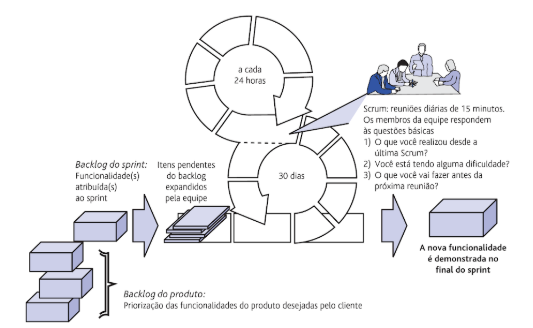
\includegraphics[width=0.95\textwidth]{img/scrum.PNG}
    \caption[Visão geral do método Scrum]{Visão geral do método Scrum. Fonte:~\cite{pressman2016engenharia}.}
    \label{fig:scrum}
\end{figure}

\subsection{Levantamento de requisitos}
\indent

O levantamento de requisitos é um meio apropriado e eficaz de entender aquilo que o cliente deseja e tem como objetivo identificar o problema, propor partes da solução, negociar diferentes abordagens e detalhar um conjunto prévio de requisitos~\citep{pressmanengenharia}. 
O levantamento de requisitos é necessário para uma boa especificação do sistema.
Um bom levantamento de requisitos pode trazer conformidade de tempo e custos do projeto de software. Para tanto, é papel do desenvolvedor insistir e enfatizar que um levantamento adequado, depende entre outros fatores, da efetiva participação do cliente na construção dos requisitos~\citep{de2003engenharia}.

\subsection{Desenvolvimento}
\indent

Depois da prototipação, do levantamento de requisitos e da escolha das tecnologias que serão utilizadas, vem a fase de construção do sistema, onde o desenvolvedor elabora e codifica a aplicação de fato, afim de corresponder ao objetivo do cliente~\citep{pressman2016engenharia}. 
Para se construir um sistema, são escritas uma série de instruções de maneira que o computador e o desenvolvedor entenda e que possa ser executado e transformado em programa~\citep{ascencio2008fundamentos}.

\subsection{Testes e Validação}
\indent

Teste é a atividade que tem como finalidade a execução do sistema de maneira monitorada, com o objetivo de estimar o seu funcionamento baseado no que foi especificado~\citep{rios2006teste}.
Durante o desenvolvimento do sistema falhas no sistema podem acontecer, ou uma funcionalidade pode ser mal construída sem que o programador perceba, com a realização de testes é possível detectar falhas ou comportamentos indesejáveis. 
É realizada a verificação do correto funcionamento das funcionalidades e a validação dos requisitos especificado pelo cliente~\citep{costa2006estrategia}.


\subsection{Implantação}
\indent

A implantação do sistema tem como característica principal a disponibilização do software em perfeito funcionamento. 
Esta é a ultima fase do projeto, que é conhecida também como "prova de fogo", pois é nessa etapa que o cliente recebe o resultado final de todo o projeto. O objetivo é realizar uma implantação com sucesso, e caso necessário elaborar manual de utilização do sistema, e realizar treinamento com o usuário final para que se obtenha a total satisfação do cliente~\citep{rezende2006engenharia}.
\chapter{Método}
\label{Metodo}
\indent

O Plano Semestral de Trabalho, como o nome sugere, é exigido dos docentes do \ac{IFG} semestralmente nos termos da Resolução nº 9 do \ac{IFG}~\citep{resolucao}.
Este capítulo descreve o trabalho efetuado para prover a solução proposta para a geração do Plano Semestral de Trabalho.

Para o gerenciamento do projeto foi empregada uma metodologia ágil inspirada no \textit{Scrum}, aplicando um sistema de entregas continuas e reuniões periódicas. 
Entretanto, os papéis de \textit{Scrum Master}, e \textit{Product Owner} não foram empregados já que a equipe se resumiu a um único desenvolvedor.
Por esta razão, a metodologia foi adaptada a fim de extrair do \textit{Scrum} as características ágeis mais adequadas ao projeto.

Inicialmente foi realizado um levantamento de requisitos funcionais com base na Resolução nº 9~\citep{resolucao} e em entrevista com o próprio orientador que é um usuário em potencial do sistema (\textit{stakeholder}).
Ao longo de \textit{Sprints} semanais, os avanços no desenvolvimento foram testados pelos \textit{stakeholders}.

%requisitos nao funcionais
Os requisitos não funcionais foram definidos a partir da proposta de melhoria na usabilidade do sistema. 
Como o sistema se propõem a ser mais completo que a planilha existente, centralizando o preenchimento dos dados e a geração do documento final, o formato \textit{Web} responsivo se mostrou uma opção viável.

O próximo passo foi desenvolver telas de protótipos com base no levantamento inicial de requisitos funcionais, os quais são apresentados na Seção~\nameref{RegrasDeNegocio}.
A Seção~\nameref{Prototipos} apresenta os protótipos iniciais, acompanhados das regras de negócio que se aplicam a cada uma das telas. 
Os protótipos foram criados utilizando a ferramenta Pencil, versão 3.0.4~\cite{pencil}. 
Depois da validação dos protótipos com o \textit{stakeholder} e criação das regras de negócio com base no levantamento de requisitos, houve material suficiente para dar início a implementação do sistema.
O protótipo inicial e as regras de negócio foram ajustados de acordo com os retornos do \textit{stakeholder} ao final de cada \textit{Sprint}.
Neste capítulo, as regras de negócio apresentadas são a versão final da documentação do sistema, enquanto os protótipos são apenas os iniciais.
No Capítulo~\nameref{Resultados} é apresentado o sistema em sua versão 1.0. 
A memória do desenvolvimento foi mantida num repositório no \href{https://github.com/waldeyr/tcc-maryana}{GitHub}\footnote{https://github.com/waldeyr/tcc-maryana}.

No desenvolvimento de uma aplicação \textit{Web}, há duas partes notadamente distintas, mas interdependentes, o \textit{back-end} e o \textit{front-end}. 

No desenvolvimento do \textit{back-end} foi utilizada a linguagem de programação \nameref{java} na versão 1.8 em conjunto do \nameref{spring} na versão 2.1.5, para a criação de uma arquitetura em camadas que está dividida na camada de domínio que é a implementação do modelo conceitual, a camada de serviço que é responsável pela a regra de negócio e que fornece operações para o~\nameref{rest}, a camada de acesso a dados que é a camada que conversa com o banco de dados~\nameref{mongo} na versão 4.0.9 e a camada de controladores~\nameref{rest} que é responsável por fornecer os dados necessários para o \textit{front-end}. 

No desenvolvimento do \textit{front-end} foi utilizado o \nameref{angular} na arquitetura e comunicação com o \textit{back-end}, como uma aplicação Angular é dividida em módulos e é baseada em componentes eles são compostos principalmente por um \textit{template} \nameref{html}, \nameref{css}, e uma classe que gerencia o componente. 
Com a criação dos componentes fornecendo a camada visual da aplicação a camada de serviço fica responsável por todas as regras de negócio da aplicação e por recuperar ou submeter dados a uma API REST. 
Foi utilizada o \nameref{bootstrap} na versão 4.3.4 para garantir o \textit{layout} responsivo para que se adapte a qualquer tamanho de tela.

Os testes e validação do sistema foram feitos pelo \textit{stakeholder} afim de verificar se os requisitos foram cumpridos e o objetivo final foi alcançado.
A implantação não ocorreu ainda e figura como trabalhos futuros através do uso de um Docker container\footnote{http://dockerhub.com} que poderá ser construído através de um Dockerfile disponível no \href{https://github.com/waldeyr/tcc-maryana}{GitHub}.

\newpage
\section{Protótipos}\label{Prototipos}
\subsection{Protótipo 01}\label{prototipo01}

A tela inicial (Protótipo 01) é mostrada na Figura~\ref{fig:prot01} e a descrição deste protótipo é mostrada na Tabela~\ref{tab:prot01}.

\begin{figure}[H]
    \centering
    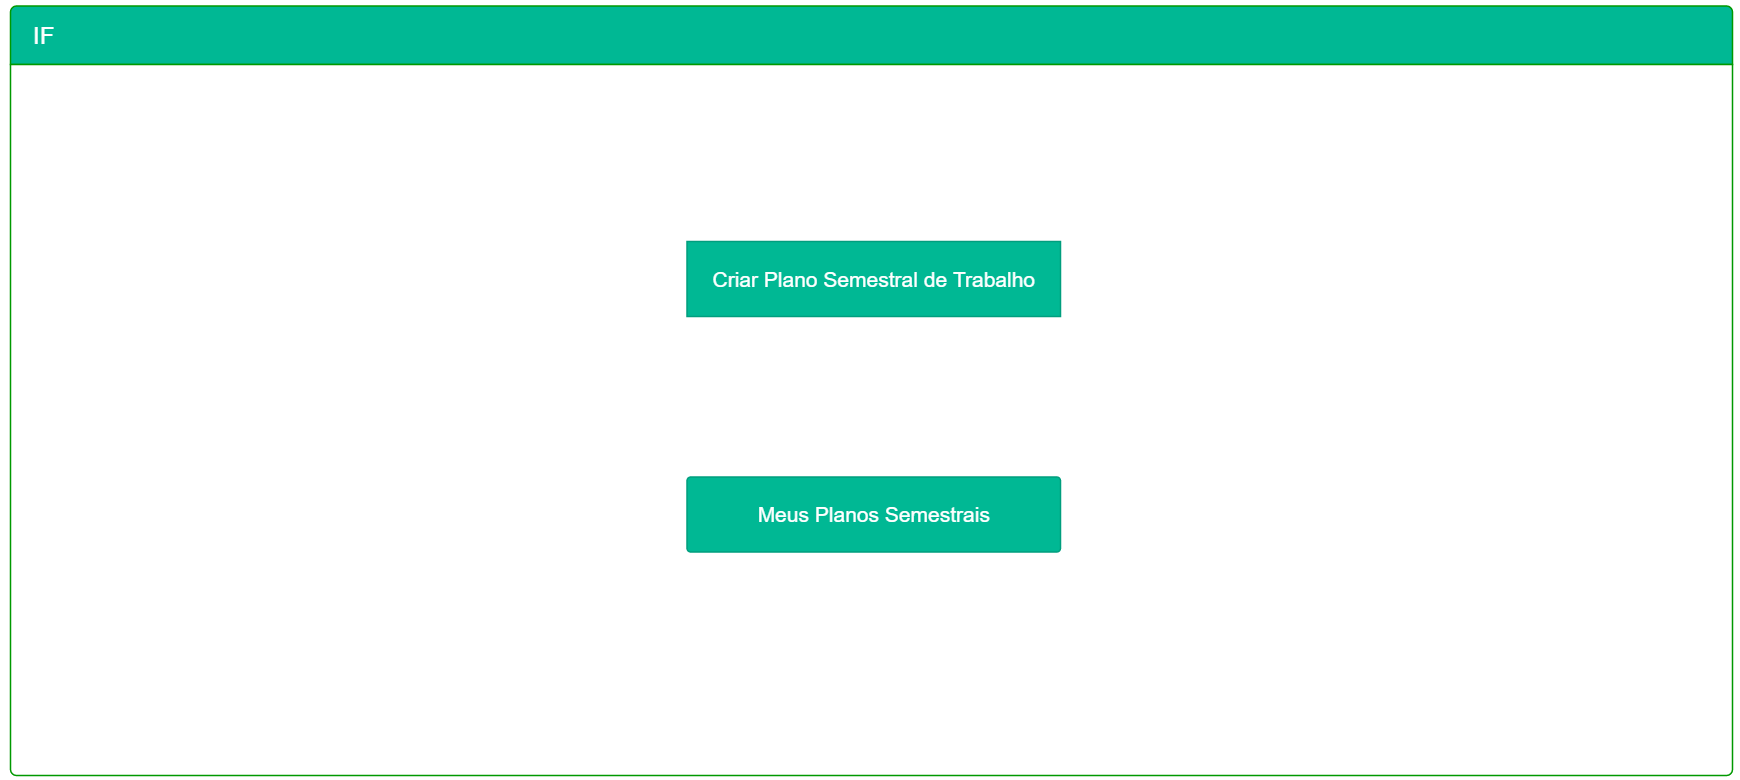
\includegraphics[width=0.95\textwidth]{img/1pagina_inicial.png}
    \caption[Protótipo 01: Tela inicial]{Protótipo 01: Tela inicial.}
    \label{fig:prot01}
\end{figure}

\begin{table}[H]
\centering
\caption[Tabela 01: Tabela descritiva do protótipo 01.]{Tabela 01: Tabela descritiva do protótipo 01.}
\label{tab:prot01}
\begin{tabular}{@{}lll@{}}
\toprule
Botões                &  Regras de Negócio                                \\ \midrule
Criar Plano Semestral de Trabalho      &     \nameref{rn016}              \\
Meus planos Semestrais                 &      \nameref{rn017}              \\ \bottomrule
\end{tabular}
\end{table}

\newpage
\subsection{Protótipo 02}\label{prototipo02}
A tela de identificação do professor (Protótipo 002) é mostrada na Figura~\ref{fig:prot02} e a descrição deste protótipo é mostrada na Tabela~\ref{tab:prot02}.


\begin{figure}[H]
    \centering
    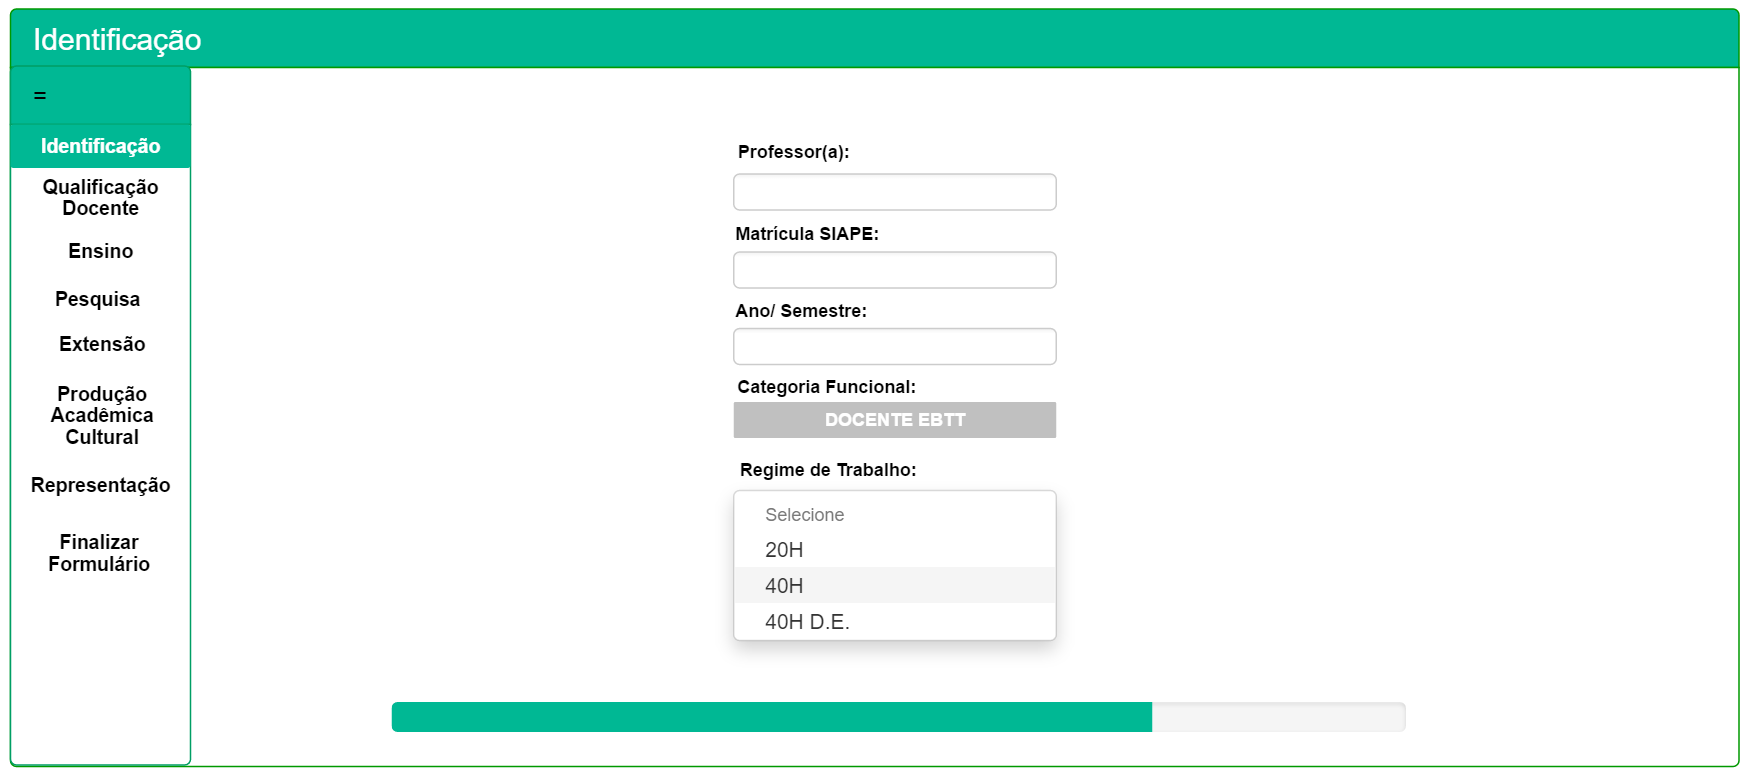
\includegraphics[width=0.95\textwidth]{img/2pagina_de_identificacao.png}
    \caption[Protótipo 02: Identificação]{Protótipo 02: Identificação.}
    \label{fig:prot02}
\end{figure}


\begin{table}[H]
\centering
\caption[Tabela 02: Tabela descritiva do protótipo 02.]{Tabela 02: Tabela descritiva do protótipo 02.}
\label{tab:prot02}
\begin{tabular}{@{}lll@{}}
\toprule
Campo               & Tipo     &  Regras de Negócio                     \\ \midrule
Professor(a)        & Texto    &    \nameref{rn002}, \nameref{rn004}    \\
Matrícula SIAPE     & Numérico &    \nameref{rn002}, \nameref{rn004}    \\
Ano/Semestre        & Texto    &    \nameref{rn002}, \nameref{rn004}    \\
Categoria Funcional & Texto    &    \nameref{rn003}, \nameref{rn004}    \\
Regime de Trabalho  & Seletor  &    \nameref{rn002}, \nameref{rn004}    \\ \bottomrule
\end{tabular}
\end{table}


\newpage
\subsection{Protótipo 03}\label{prototipo03}
A tela de qualificação do docente (Protótipo 03) é mostrada na Figura~\ref{fig:prot03} e a descrição deste protótipo é mostrada na Tabela~\ref{tab:prot03}.


\begin{figure}[H]
    \centering
    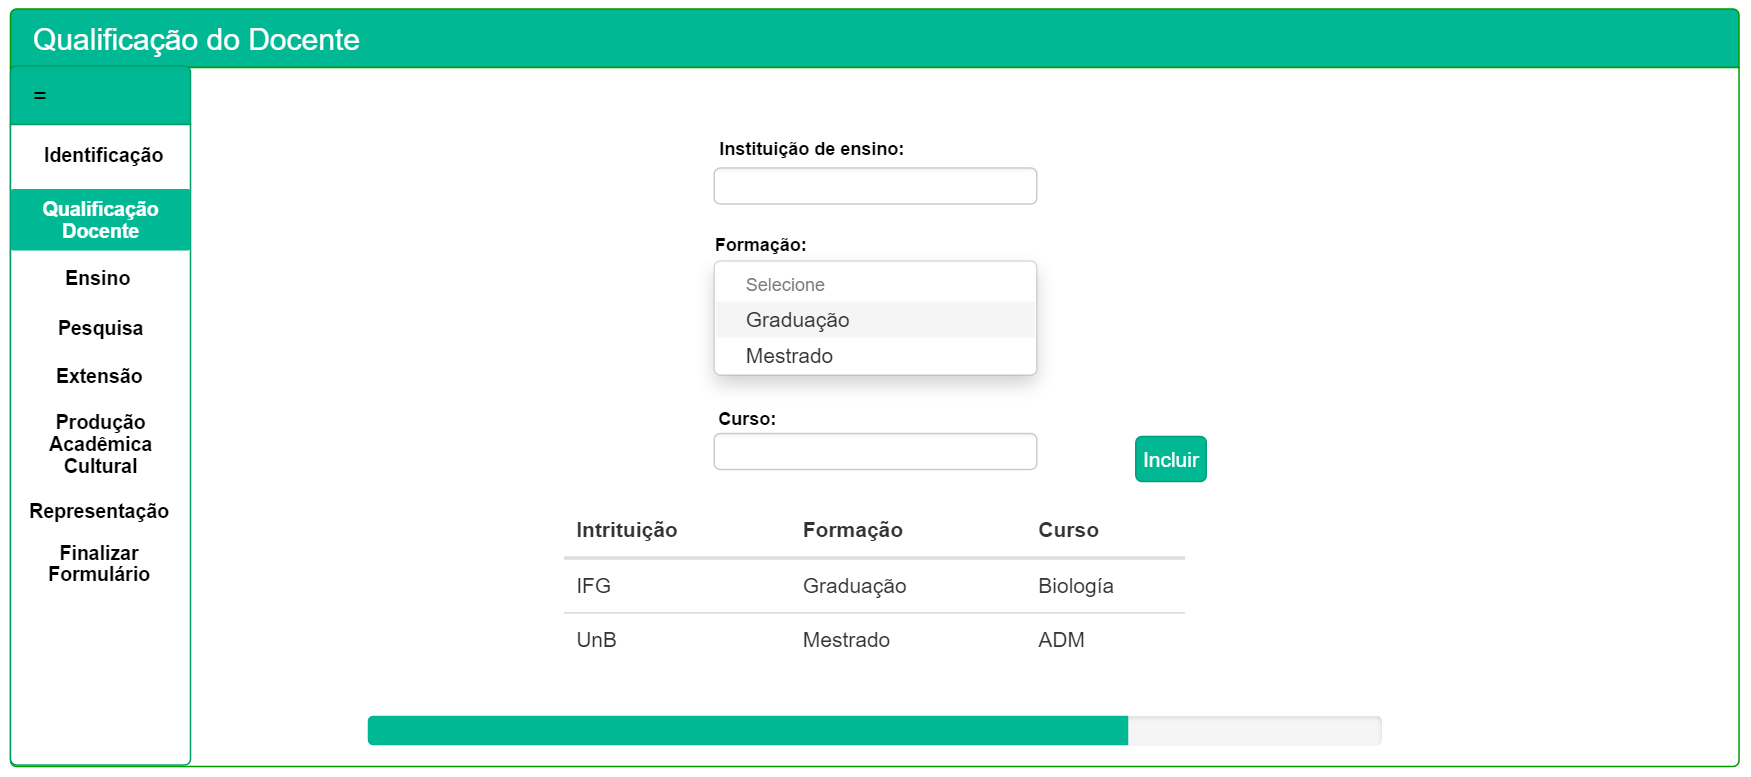
\includegraphics[width=0.95\textwidth]{img/3pagina_qualificacao_do_docente.png}
    \caption[Protótipo 03: Qualificação do Docente]{Protótipo 03: Qualificação do Docente.}
    \label{fig:prot03}
\end{figure}


\begin{table}[H]
\centering
\caption[Tabela 03: Tabela descritiva do protótipo 03.]{Tabela 03: Tabela descritiva do protótipo 03.}
\label{tab:prot03}
\begin{tabular}{@{}lll@{}}
\toprule
Campo                   & Tipo     &  Regras de Negócio                     \\ \midrule
Instituição de ensino   & Texto    &    \nameref{rn005}, \nameref{rn006}    \\
Formação                & Seletor  &    \nameref{rn005}, \nameref{rn006}    \\
Curso                   & Texto    &    \nameref{rn005}, \nameref{rn006}    \\ \bottomrule
\end{tabular}
\end{table}

\newpage
\subsection{Protótipo 04}\label{prototipo04}
A tela de atividades de ensino (Protótipo 04) é mostrada na Figura~\ref{fig:prot04} e a descrição deste protótipo é mostrada na Tabela~\ref{tab:prot04}.

\begin{figure}[H]
    \centering
    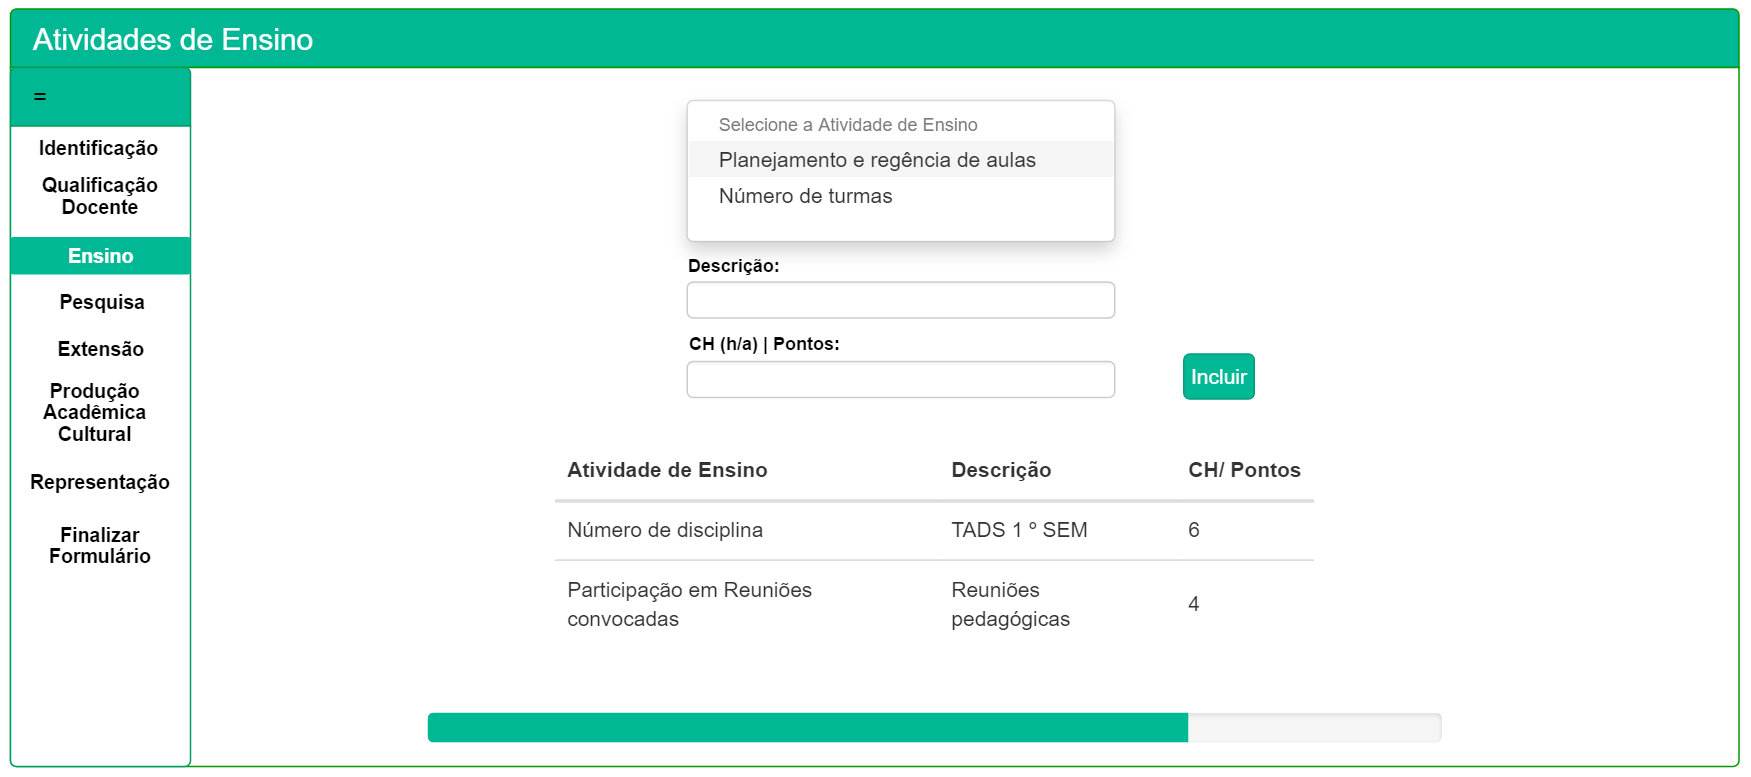
\includegraphics[width=0.95\textwidth]{img/4pagina_atividades_de_ensino.png}
    \caption[Protótipo 04: Atividade de Ensino]{Protótipo 04: Atividade de Ensino.}
    \label{fig:prot04}
\end{figure}

\begin{table}[H]
\centering
\caption[Tabela 04: Tabela descritiva do protótipo 04.]{Tabela 04: Tabela descritiva do protótipo 04.}
\label{tab:prot04}
\begin{tabular}{@{}lll@{}}
\toprule
Campo                           & Tipo     &  Regras de Negócio             \\ \midrule
Selecione a Atividade de Ensino & Seletor  &    \nameref{rn007}, \nameref{rn019}     \\
Descrição                       & Texto    &    \nameref{rn007}                 \\
CH(h/a)|Pontos:                 & Numérico &    \nameref{rn007}, \nameref{rn020}     \\ \bottomrule
\end{tabular}
\end{table}

\newpage
\subsection{Protótipo 05}\label{prototipo05}
A tela de atividades de pesquisa (Protótipo 05) é mostrada na Figura~\ref{fig:prot05} e a descrição deste protótipo é mostrada na Tabela~\ref{tab:prot05}.


\begin{figure}[H]
    \centering
    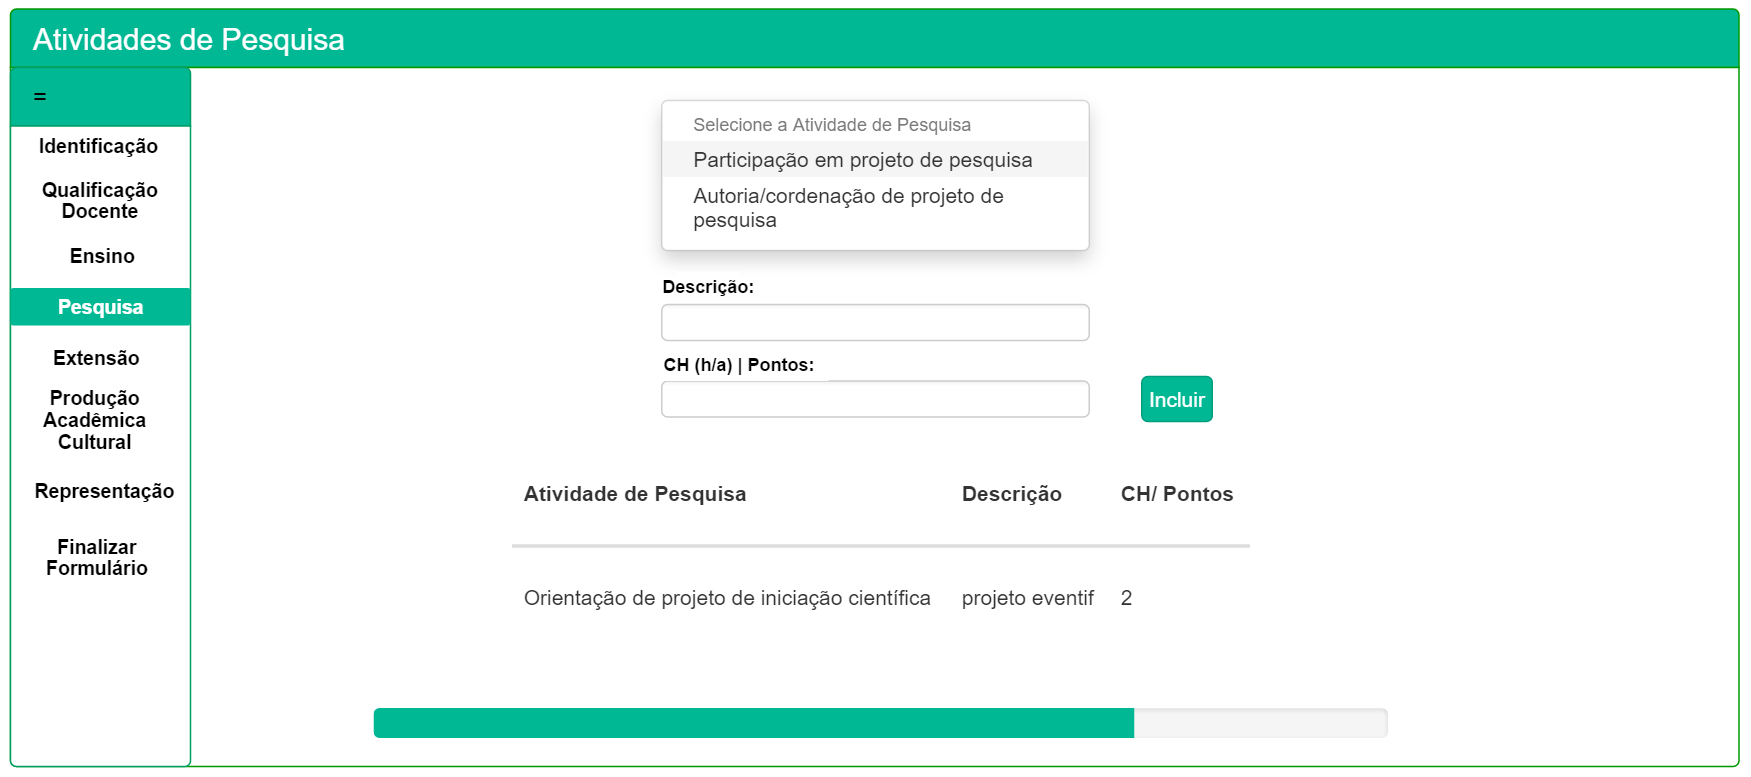
\includegraphics[width=0.95\textwidth]{img/5pagina_pesquisa.png}
    \caption[Protótipo 05: Atividade de Pesquisa]{Protótipo 05: Atividade de Pesquisa.}
    \label{fig:prot05}
\end{figure}


\begin{table}[H]
\centering
\caption[Tabela 05: Tabela descritiva do protótipo 05.]{Tabela 05: Tabela descritiva do protótipo 05.}
\label{tab:prot05}
\begin{tabular}{@{}lll@{}}
\toprule
Campo                             & Tipo     &  Regras de Negócio     \\ \midrule
Selecione a Atividade de Pesquisa & Seletor  &    \nameref{rn008}, \nameref{rn019}\\
Descrição                         & Texto    &    \nameref{rn008}                 \\
CH(h/a)|Pontos:                   & Numérico &    \nameref{rn008}, \nameref{rn020}\\ \bottomrule
\end{tabular}
\end{table}

\newpage
\subsection{Protótipo 06}\label{prototipo06}
A tela de atividades de extensão (Protótipo 06) é mostrada na Figura~\ref{fig:prot06} e a descrição deste protótipo é mostrada na Tabela~\ref{tab:prot06}.


\begin{figure}[H]
    \centering
    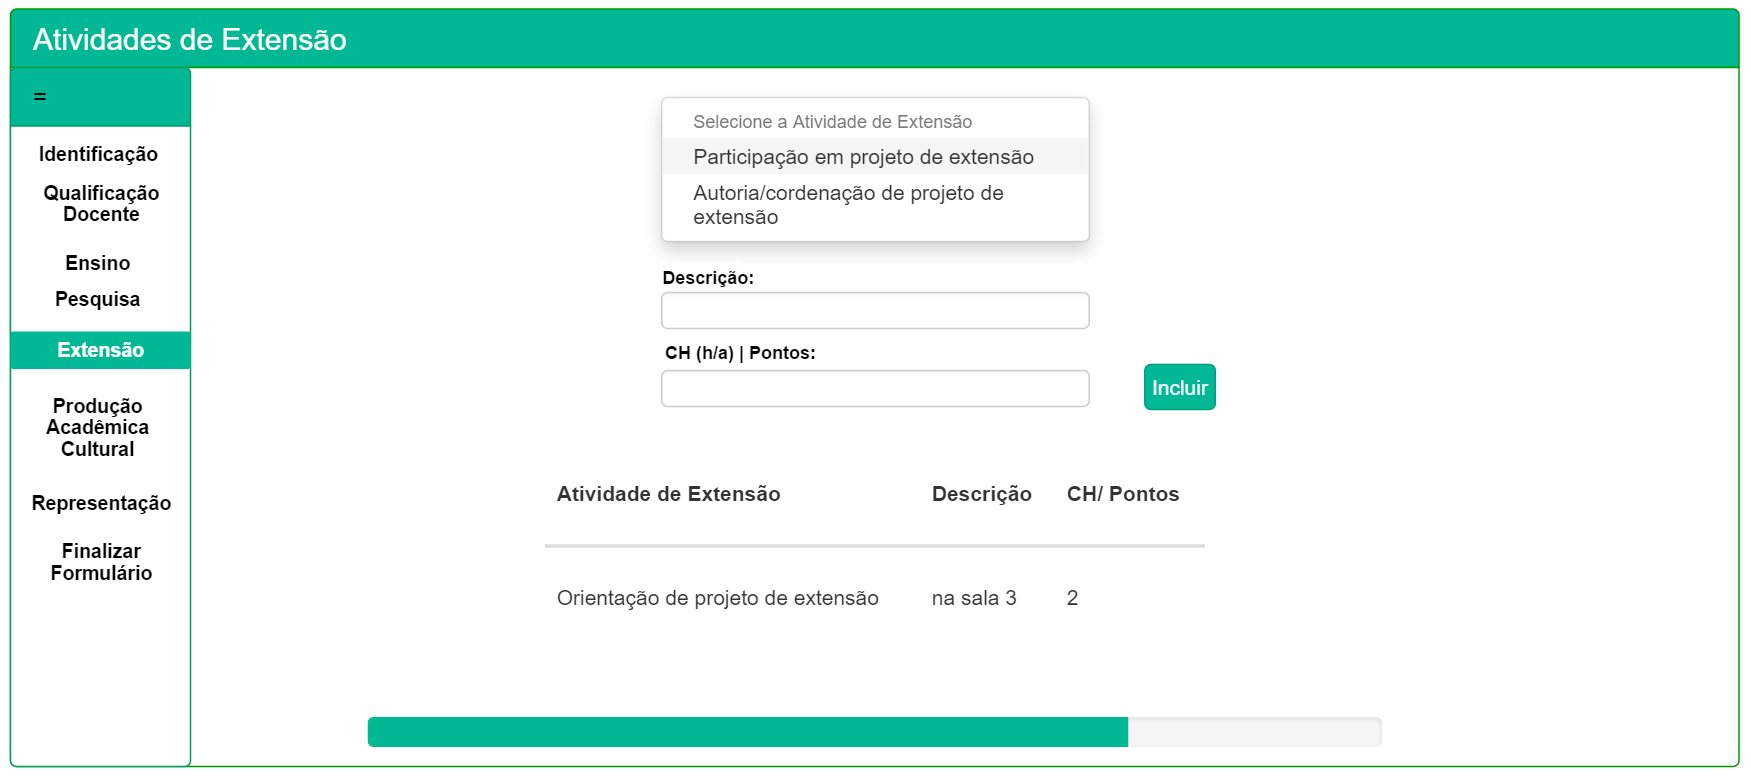
\includegraphics[width=0.95\textwidth]{img/6pagina_extensao.png}
    \caption[Protótipo 06: Atividade de Extensão]{Protótipo 06: Atividade de Extensão.}
    \label{fig:prot06}
\end{figure}


\begin{table}[H]
\centering
\caption[Tabela 06: Tabela descritiva do protótipo 06.]{Tabela 06: Tabela descritiva do protótipo 06.}
\label{tab:prot06}
\begin{tabular}{@{}lll@{}}
\toprule
Campo                             & Tipo     &  Regras de Negócio     \\ \midrule
Selecione a Atividade de Extensão & Seletor  &    \nameref{rn009}, \nameref{rn019}\\
Descrição                         & Texto    &    \nameref{rn009}                 \\
CH(h/a)|Pontos:                   & Numérico &    \nameref{rn009}, \nameref{rn020}\\ \bottomrule
\end{tabular}
\end{table}

\newpage
\subsection{Protótipo 07}\label{prototipo07}
A tela de atividades de produção acadêmica cultural (Protótipo 07) é mostrada na Figura~\ref{fig:prot07} e a descrição deste protótipo é mostrada na Tabela~\ref{tab:prot07}.


\begin{figure}[H]
    \centering
    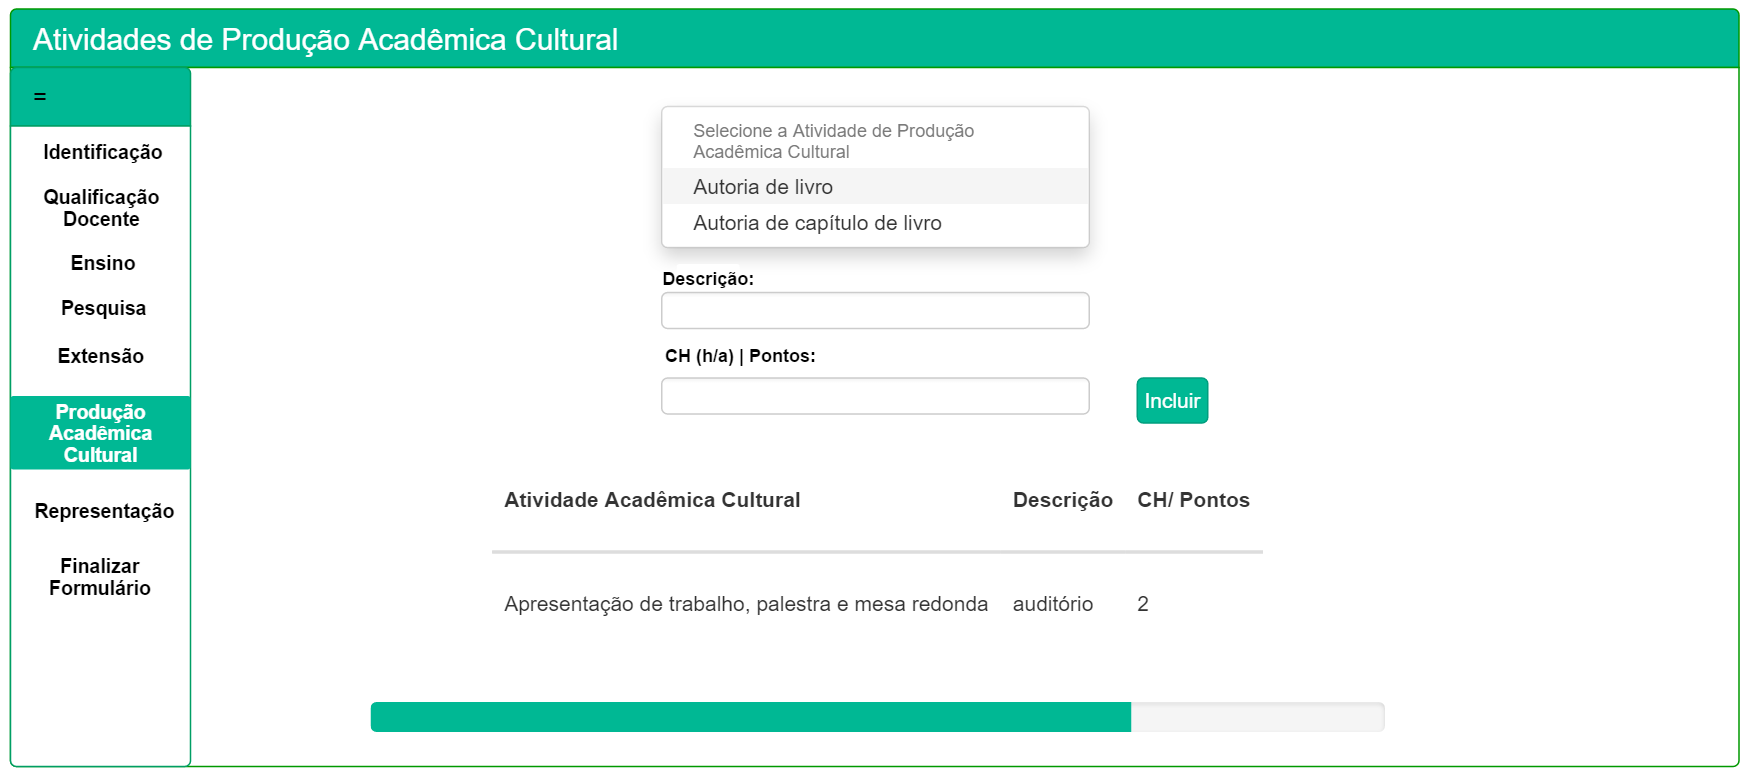
\includegraphics[width=0.95\textwidth]{img/7pagina_de_prod_academica.png}
    \caption[Protótipo 07: Atividade de Produção Acadêmica Cultural]{Protótipo 07: Atividade de Produção Acadêmica Cultural.}
    \label{fig:prot07}
\end{figure}


\begin{table}[H]
\centering
\caption[Tabela 07: Tabela descritiva do protótipo 07.]{Tabela 07: Tabela descritiva do protótipo 07.}
\label{tab:prot07}
\begin{tabular}{@{}lll@{}}
\toprule
Campo                                                & Tipo     &  Regras de Negócio     \\ \midrule
Selecione a Atividade de Produção Acadêmica Cultural & Seletor  &    \nameref{rn010}, \nameref{rn019}\\
Descrição                                            & Texto    &    \nameref{rn010}                 \\
CH(h/a)|Pontos:                                      & Numérico &    \nameref{rn010}, \nameref{rn020}\\ \bottomrule
\end{tabular}
\end{table}

\newpage
\subsection{Protótipo 08}\label{prototipo08}

A tela de atividades de representação (Protótipo 08) é mostrada na Figura~\ref{fig:prot08} e a descrição deste protótipo é mostrada na Tabela~\ref{tab:prot08}.

\begin{figure}[H]
    \centering
    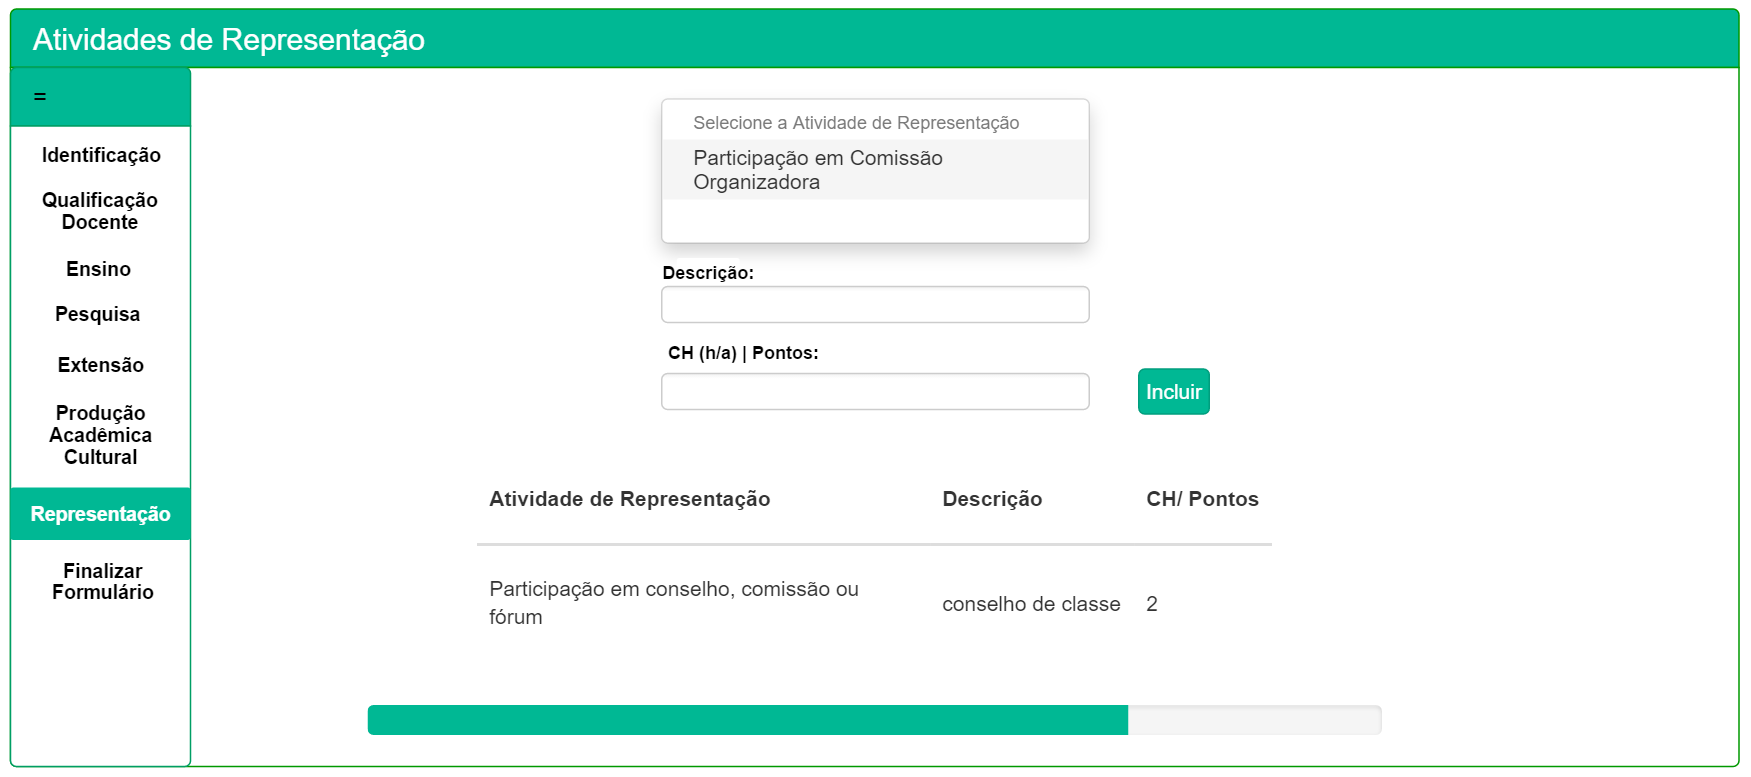
\includegraphics[width=0.95\textwidth]{img/8pagina_representacao.png}
    \caption[Protótipo 08: Atividade de Representação]{Protótipo 08: Atividade de Representação.}
    \label{fig:prot08}
\end{figure}


\begin{table}[H]
\centering
\caption[Tabela 08: Tabela descritiva do protótipo 08.]{Tabela 08: Tabela descritiva do protótipo 08.}
\label{tab:prot08}
\begin{tabular}{@{}lll@{}}
\toprule
Campo                                   & Tipo     &  Regras de Negócio     \\ \midrule
Selecione a Atividade de Representação  & Seletor  &    \nameref{rn011}, \nameref{rn019}\\
Descrição                               & Texto    &    \nameref{rn011}                 \\
CH(h/a)|Pontos:                         & Numérico &    \nameref{rn011}, \nameref{rn020}\\ \bottomrule
\end{tabular}
\end{table}

\newpage
\subsection{Protótipo 09}\label{prototipo09}
A tela de finalizar o formulário (Protótipo 09) é mostrada na Figura~\ref{fig:prot09} e a descrição deste protótipo é mostrada na Tabela~\ref{tab:prot09}.


\begin{figure}[H]
    \centering
    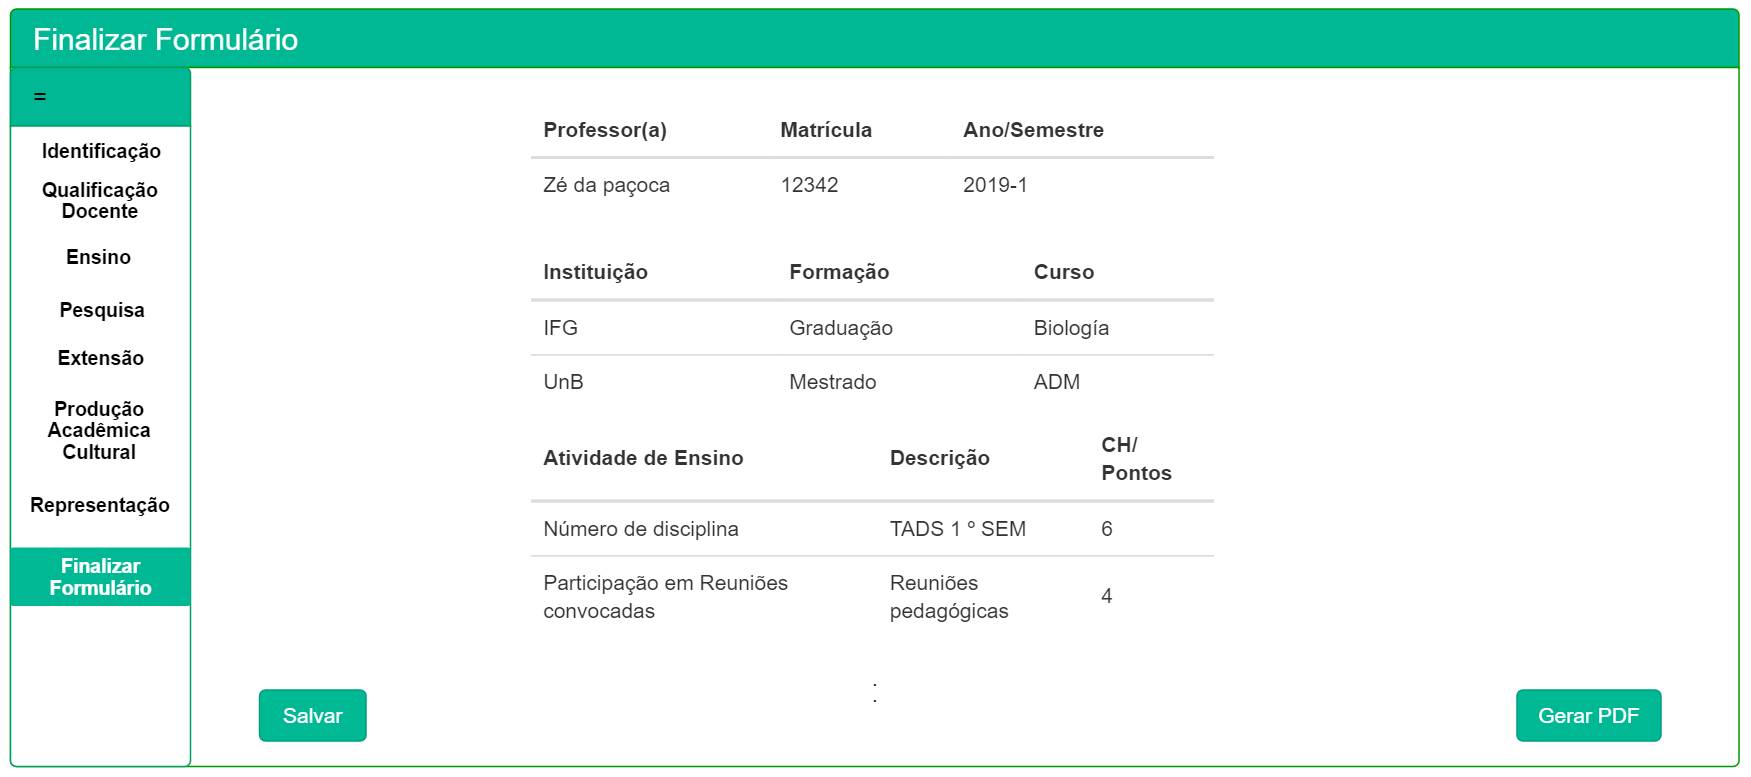
\includegraphics[width=0.95\textwidth]{img/9pagina_finalizar_formulario.png}
    \caption[Protótipo 09: Finalizar Formulário]{Protótipo 09: Finalizar Formulário.}
    \label{fig:prot09}
\end{figure}


\begin{table}[H]
\centering
\caption[Tabela 09: Tabela descritiva do protótipo 09.]{Tabela 09: Tabela descritiva do protótipo 09.}
\label{tab:prot09}
\begin{tabular}{@{}lll@{}}
\toprule
Botões      &  Regras de Negócio                                \\ \midrule
Salvar      &     \nameref{rn012}, \nameref{rn015}              \\
Gerar PDF   &     \nameref{rn012}, \nameref{rn014}              \\ \bottomrule
\end{tabular}
\end{table}



\newpage
\section{Regras de Negócio}\label{RegrasDeNegocio}

\subsection{RN001}\label{rn001}

O usuário deve ser um professor(a) do IFG.

\subsection{RN002}\label{rn002}

O usuário deve informar no menu ``Identificação'' os seguintes dados: Nome, matrícula SIAPE, ano/semestre, \textit{e-mail} e regime de trabalho.

\subsection{RN003}\label{rn003}

A informação sobre a categoria funcional do usuário deve ser incluída por padrão pelo sistema. Esse valor deve ser: DOCENTE EBTT.

\subsection{RN004}\label{rn004}

Todos os campos do menu ``Identificação'' são obrigatórios. 

\subsection{RN005}\label{rn005}

O usuário deve informar no menu ``Qualificação do Docente'' os seguintes dados: Instituição de ensino, formação e curso.

\subsection{RN006}\label{rn006}

Todos os campos do menu ``Qualificação do Docente'' são obrigatórios. 

\subsection{RN007}\label{rn007}

O usuário deve informar no menu ``Ensino'' os seguintes dados: A atividade de ensino, descrição e a carga horária ou pontuação. 

\subsection{RN008}\label{rn008}

O usuário deve informar no menu ``Pesquisa'' os seguintes dados: A atividade de pesquisa, descrição e a carga horária ou pontuação. 

\subsection{RN009}\label{rn009}

O usuário deve informar no menu ``Extensão'' os seguintes dados: A atividade de extensão, descrição e a carga horária ou pontuação.

\subsection{RN010}\label{rn010}

O usuário deve informar no menu ``Produção Acadêmica Cultural'' os seguintes dados: A atividade de produção acadêmica cultural, descrição e a carga horária ou pontuação.

\subsection{RN011}\label{rn011}

O usuário deve informar no menu ``Atividade de Qualificação'' os seguintes dados: A atividade de qualificação, descrição e a carga horária ou pontuação.

\subsection{RN012}\label{rn012}

O usuário deve informar no menu ``Representação'' os seguintes dados: A atividade de representação, descrição e a carga horária ou pontuação.

\subsection{RN013}\label{rn013}

O usuário deve verificar as informações de seu formulário no menu ``Finalizar Formulário''.

\subsection{RN014}\label{rn014}

O usuário deve ter uma somatória de pontos correspondente a carga horária do regime de trabalho preenchida na regra de negócio [\nameref{rn002}]

\subsection{RN015}\label{rn015}

No menu ``Finalizar Formulário'' o usuário deve clicar no botão ``Gerar PDF'' para gerar o \ac{PDF} do formulário plano semestral de trabalho.

\subsection{RN016}\label{rn016}

No menu ``Finalizar Formulário'' o usuário deve clicar no botão "Salvar" para salvar o formulário plano semestral de trabalho.

\subsection{RN017}\label{rn017}

Na página inicial o usuário deve clicar no botão ``Criar Plano Semestral de Trabalho'' para iniciar o formulário.

\subsection{RN018}\label{rn018}

Na página inicial o usuário deve clicar no botão ``Meus Planos Semestrais'' para recuperar um formulário já existente.

\subsection{RN019}\label{rn019}

A atividade de uma categoria só pode ser selecionada uma vez, então o usuário deve preencher  na descrição todo o conteúdo relacionada com aquela determinada atividade, e no campo de carga horária ou pontuação preencher com o valor total destinado para a atividade em questão.

\subsection{RN020}\label{rn020}

O campo de carga horária ou pontuação tem valor máximo limitado de acordo com a Resolução 9~\citep{resolucao}.

\subsection{RN021}\label{rn021}

A tabela com a listagem de todas as atividades, pontuação e somatório encontra se na página de finalização do formulário.


\chapter{Resultados}
\label{Resultados}

O Plano Semestral de Trabalho dos Docentes do \ac{IFG} é um documento que precisa ser impreterivelmente confeccionado e entregue à Chefia do Departamento de Áreas Acadêmicas dos \textit{campi}.
O documento é normatizado nos termos da Resolução 09 de 1º de Novembro de 2011 do \ac{IFG}~\citep{resolucao}.
Este Trabalho de Conclusão de Curso, conforme definido no objetivo, almejou construir uma solução \textit{user-friendly} e independente de sistema operacional para a elaboração do Plano Semestral de Trabalho nos termos da Resolução 09 de 1º de Novembro de 2011 do \ac{IFG}.

A partir da prototipação como metodologia de desenvolvimento de software, utilizando tecnologias de desenvolvimento \textit{Web}, um banco de dados \ac{NoSQL} baseado em documentos e SCRUM como metodologia de gerenciamento do projeto, foi construída uma aplicação \textit{web} para o preenchimento do documento ``Plano Semestral de Trabalho Docente'' de acordo com a Resolução nº 09 de 1º de Novembro de 2011~\citep{resolucao}.

A aplicação funciona em qualquer browser e se ajusta de forma automática ao tamanho da tela do usuário, o que a torna independente de sistema operacional.
Além disso, a usabilidade da aplicação foi ajustada atualizando o layout conforme solicitações dos \textit{stakeholders} ao final de cada \textit{Sprint}.
Tais ajustes atualizaram tanto o protótipo inicial, quanto as regras de negócio.

Os resultados são apresentados neste texto sob a forma de figuras das telas do sistema, o qual está em sua versão inicial (1.0) disponível para implantação por parte do \textit{campus} Formosa do \ac{IFG}.
A Figura \ref{fig:result01} mostra a tela inicial do sistema no qual foi adicionado um botão de início do \nameref{fig:prot01}, para melhorar a navegação.
A Figura \ref{fig:result02} mostra a tela de identificação do usuário, o campo \textit{e-mail} foi adicionado do \nameref{fig:prot02}, para futuramente ser possível enviar \textit{e-mail} para o usuário com o link de busca do formulário.
A Figura \ref{fig:result03} mostra a tela de cadastro da qualificação do docente.
A Figura \ref{fig:result04} mostra a tela de cadastro de atividades de ensino.
A Figura \ref{fig:result05} mostra a tela de cadastro de atividades de pesquisa.
A Figura \ref{fig:result06} mostra a tela de cadastro de atividades de extensão.
A Figura \ref{fig:result07} mostra a tela de cadastro de atividades de produção acadêmica e cultural.
A Figura \ref{fig:result08} mostra a tela de cadastro de atividades de qualificação, que não havia sido prototipada.
A Figura \ref{fig:result09} mostra a tela de cadastro de atividades de representação.
A Figura \ref{fig:result10} mostra a tela de finalização do formulário.
A Figura \ref{fig:result11} mostra a mensagem de que o formulário foi salvo com sucesso.
A Figura \ref{fig:result12} mostra a tela de busca do formulário.

\begin{figure}[htb]
    \centering
    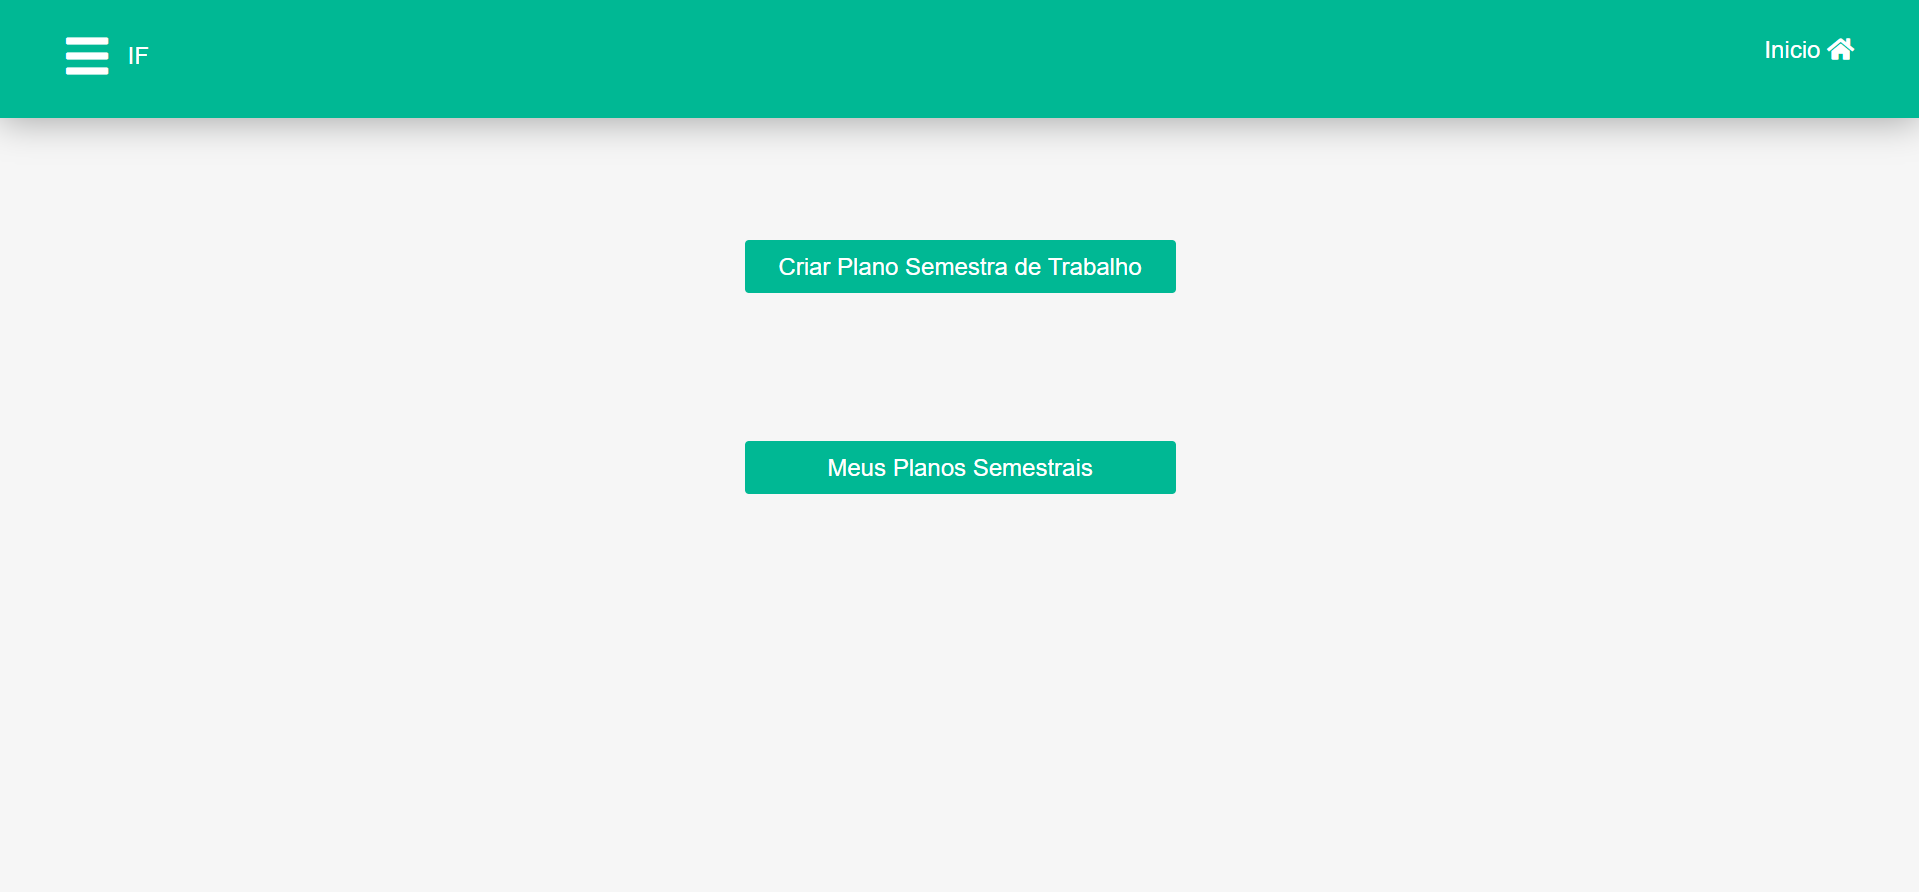
\includegraphics[width=.99\textwidth]{img/pagina_inicial.PNG}
    \caption[Resultado 01: Tela inicial]{Resultado 01: Tela inicial.}
    \label{fig:result01}
\end{figure}

\begin{figure}[htb]
    \centering
    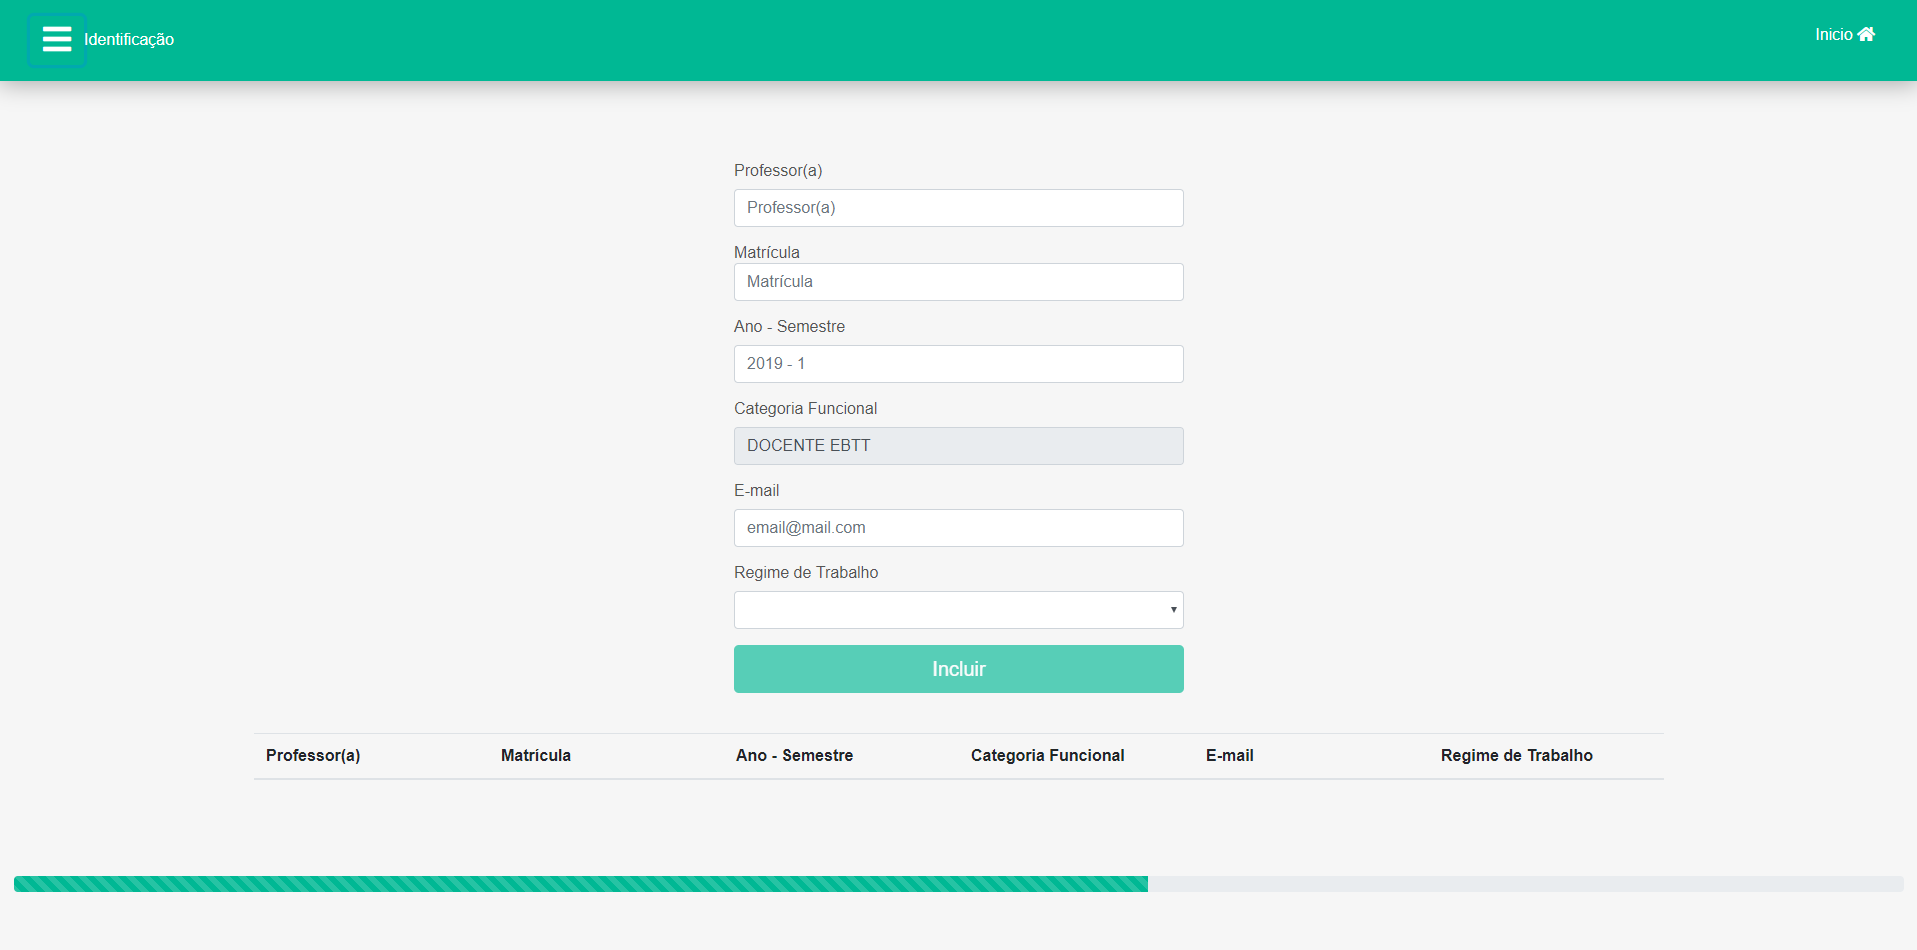
\includegraphics[width=.99\textwidth]{img/pagina_identificacao.PNG}
    \caption[Resultado 02: Tela de Identificação]{Resultado 02: Tela de Identificação.}
    \label{fig:result02}
\end{figure}

\begin{figure}[htb]
    \centering
    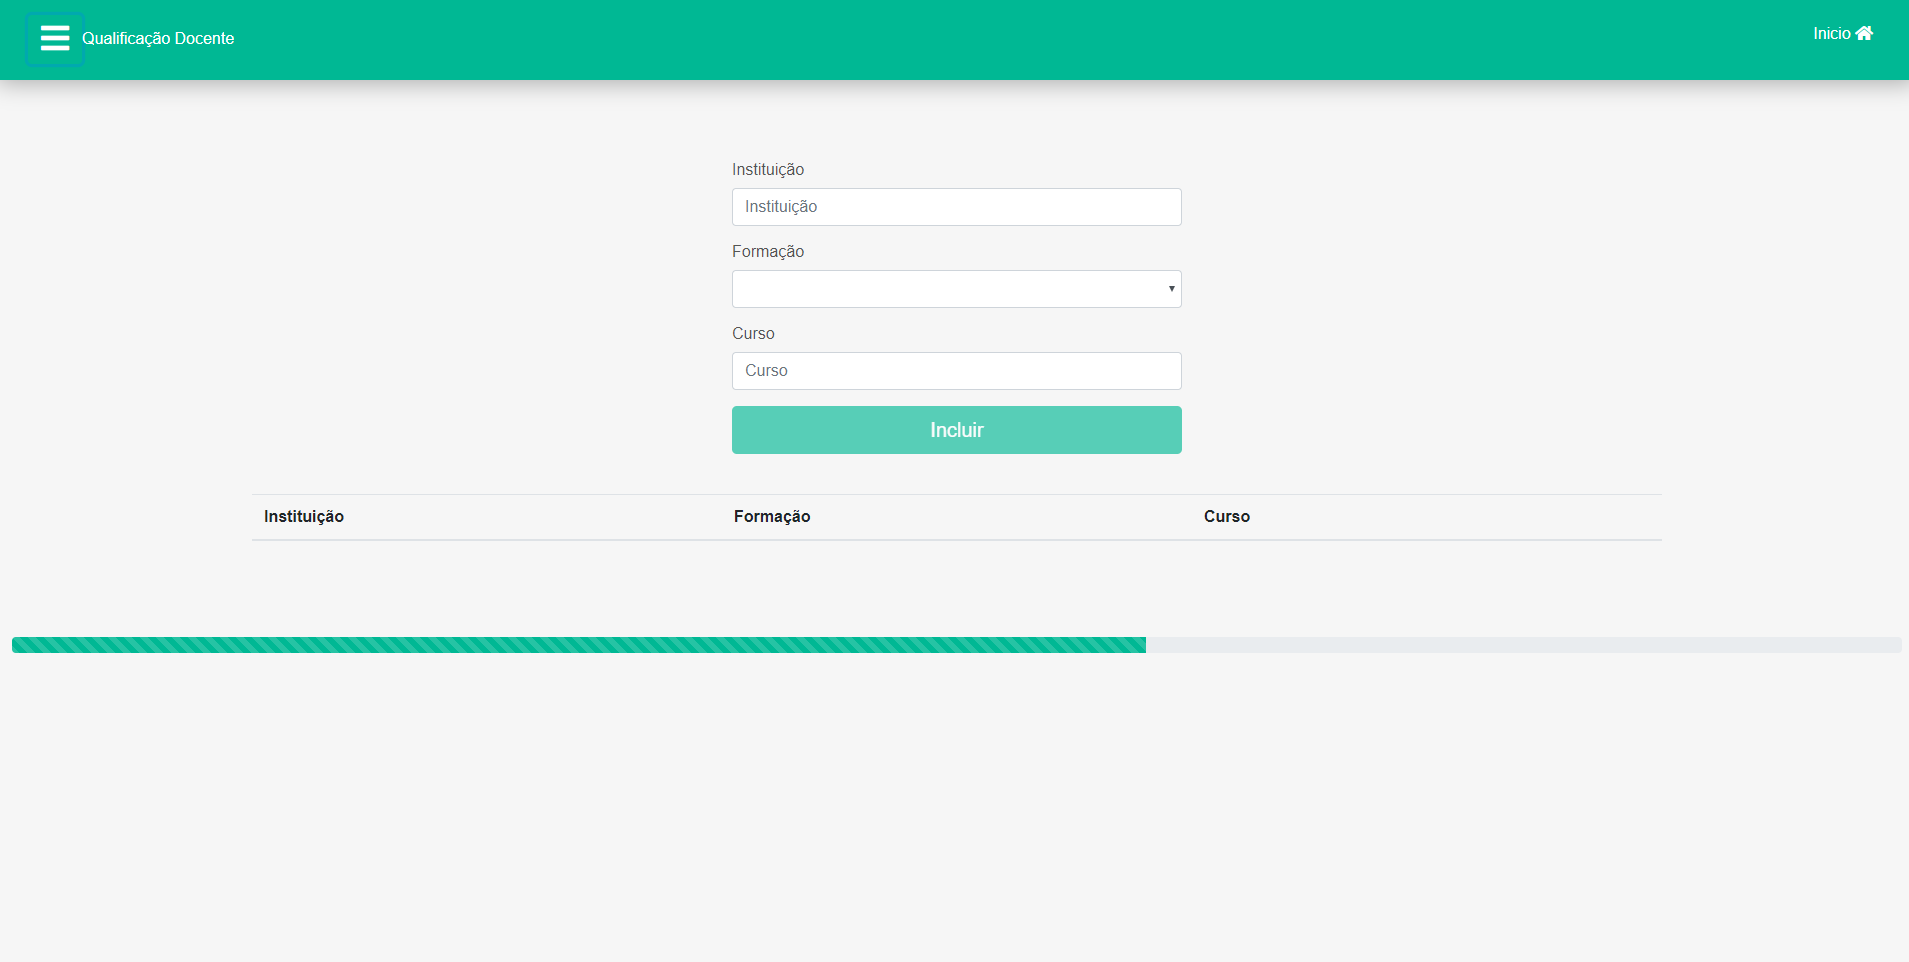
\includegraphics[width=.8\textwidth]{img/pagina_qualificacao_docente.PNG}
    \caption[Resultado 03: Tela de Qualificação do Docente]{Resultado 03: Tela de Qualificação do Docente.}
    \label{fig:result03}
\end{figure}

\begin{figure}[htb]
    \centering
    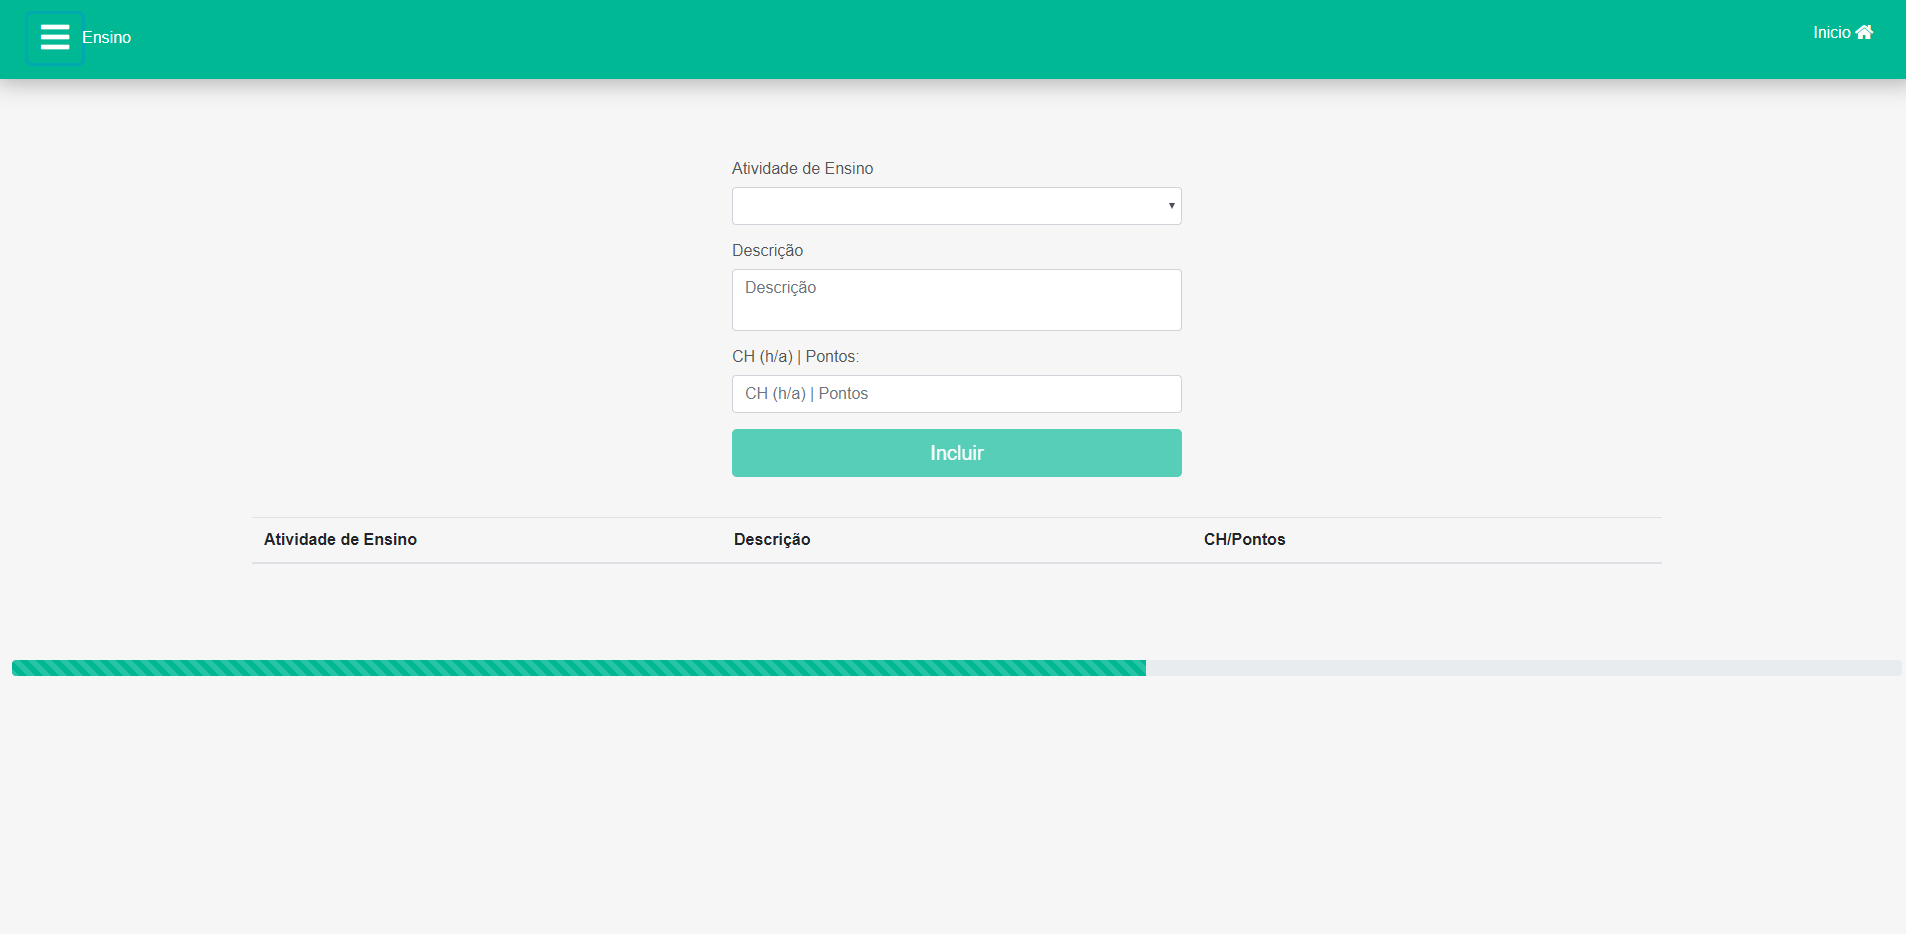
\includegraphics[width=.8\textwidth]{img/pagina_ensino.PNG}
    \caption[Resultado 04: Tela de Atividades de Ensino]{Resultado 04: Tela de Atividades de Ensino.}
    \label{fig:result04}
\end{figure}

\begin{figure}[htb]
    \centering
    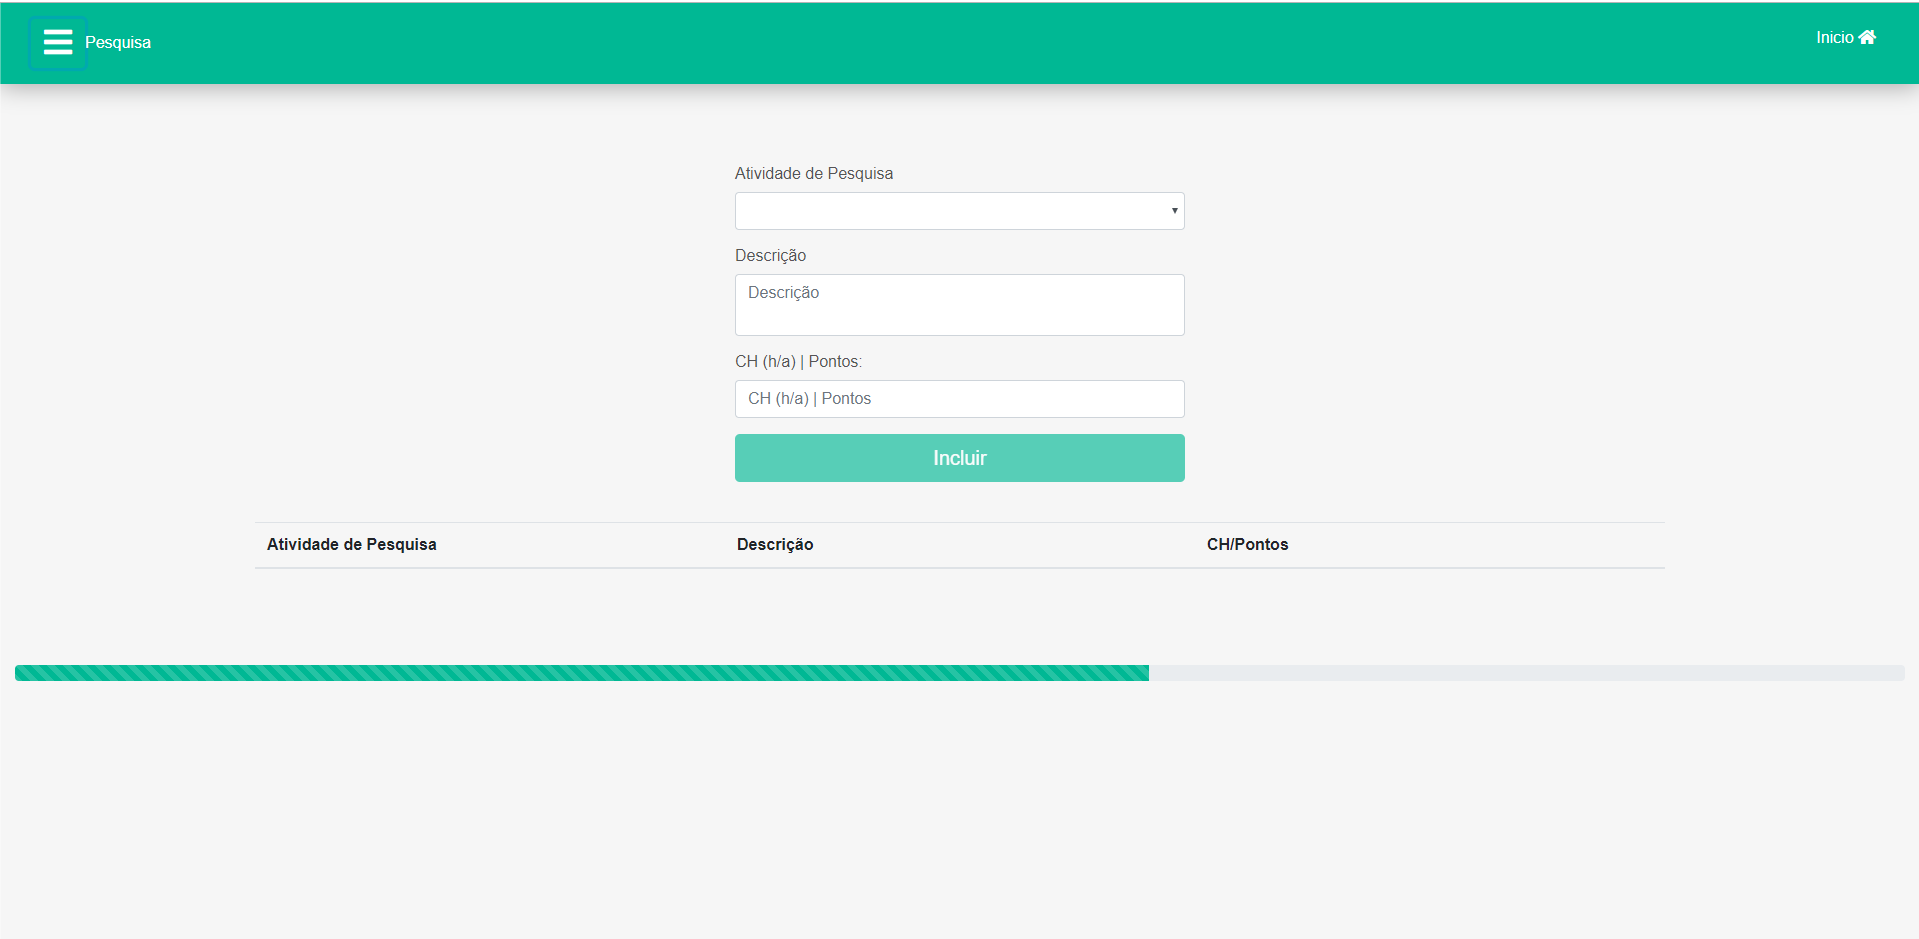
\includegraphics[width=.8\textwidth]{img/pagina_pesquisa.PNG}
    \caption[Resultado 05: Tela de Atividades de Pesquisa]{Resultado 05: Tela de Atividades de Pesquisa.}
    \label{fig:result05}
\end{figure}

\begin{figure}[htb]
    \centering
    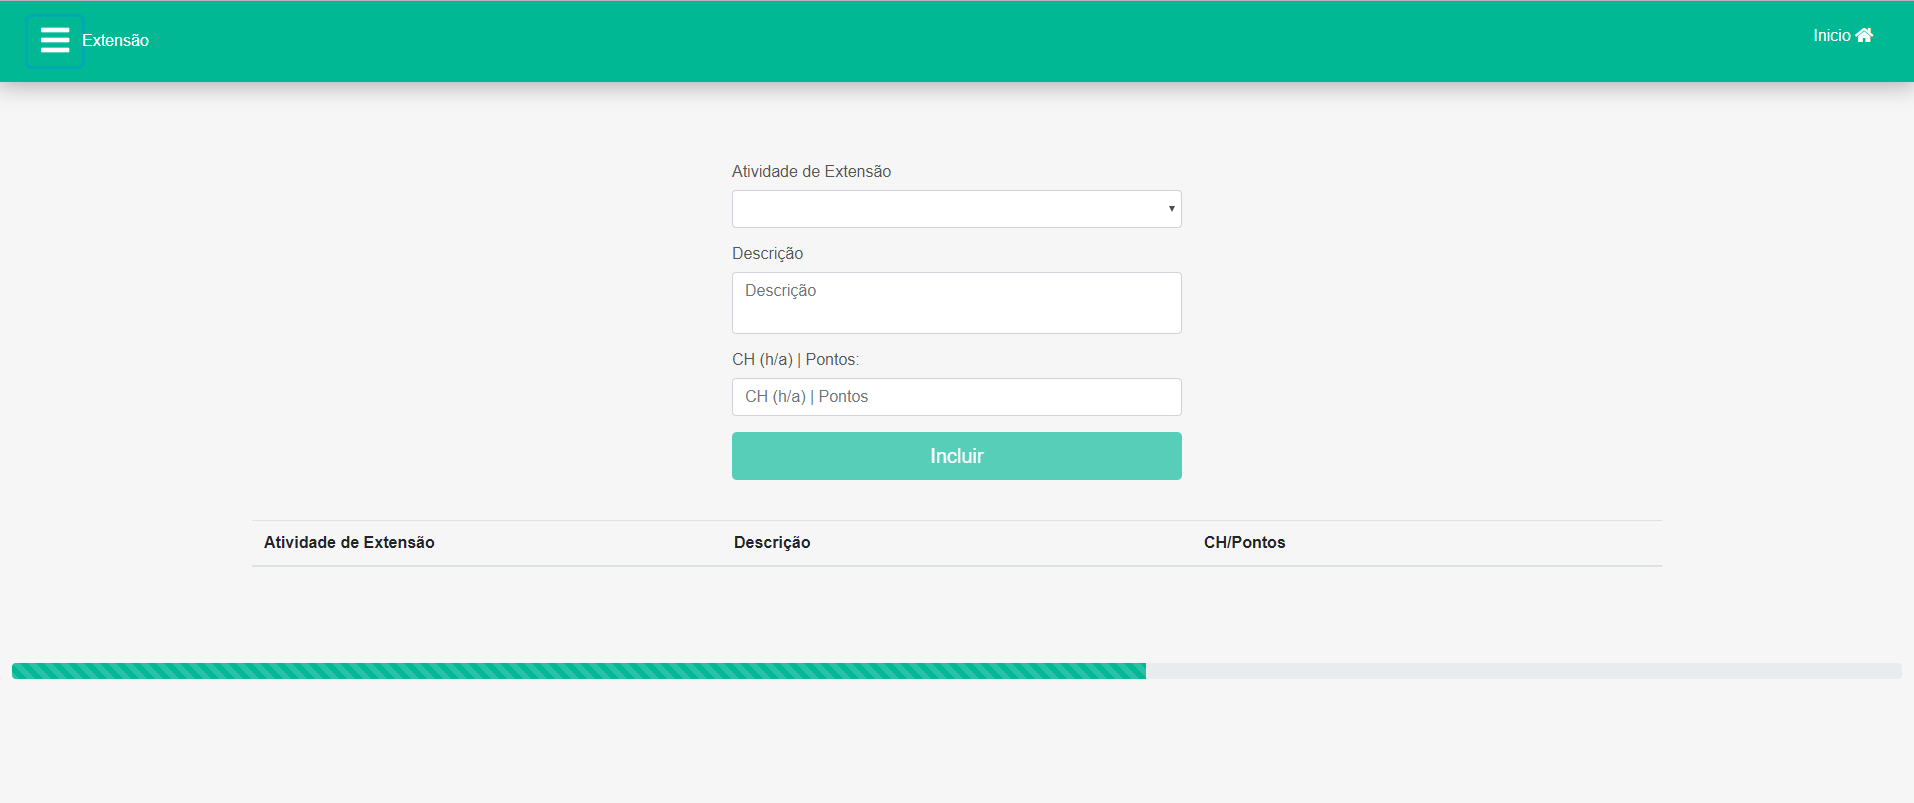
\includegraphics[width=.8\textwidth]{img/pagina_extensao.PNG}
    \caption[Resultado 06: Tela de Atividades de Extensão]{Resultado 06: Tela de Atividades de Extensão.}
    \label{fig:result06}
\end{figure}

\begin{figure}[htb]
    \centering
    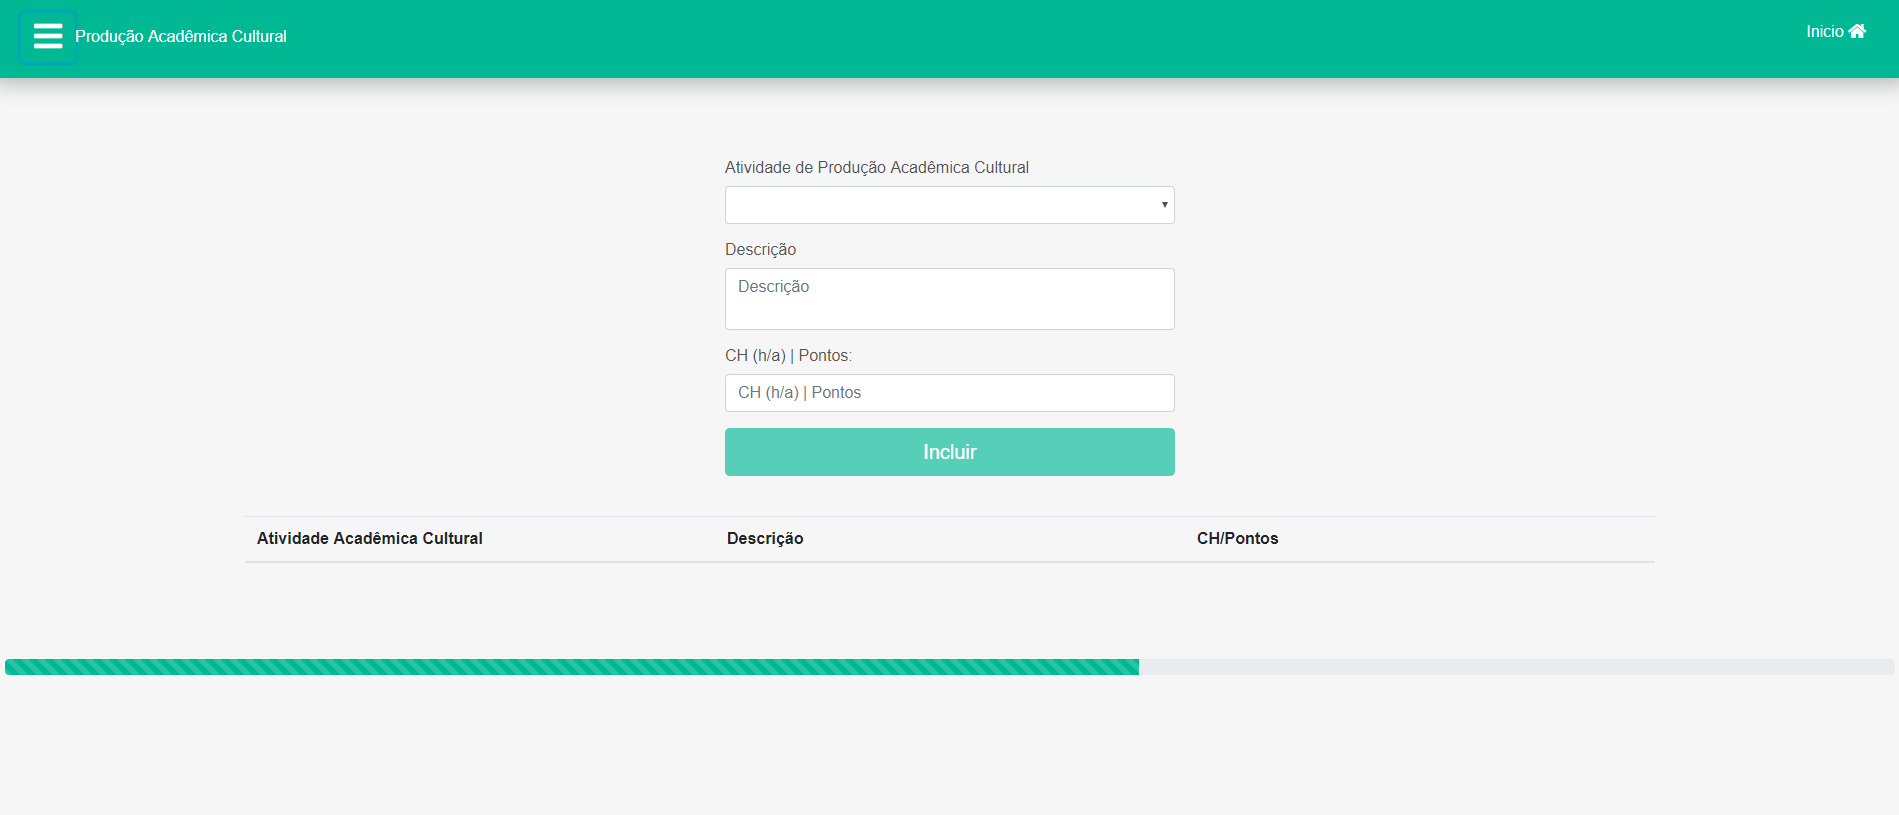
\includegraphics[width=.8\textwidth]{img/pagina_producao.PNG}
    \caption[Resultado 07: Tela de Atividades de Produção Acadêmica]{Resultado 07: Tela de Atividades de Produção Acadêmica.}
    \label{fig:result07}
\end{figure}

\begin{figure}[htb]
    \centering
    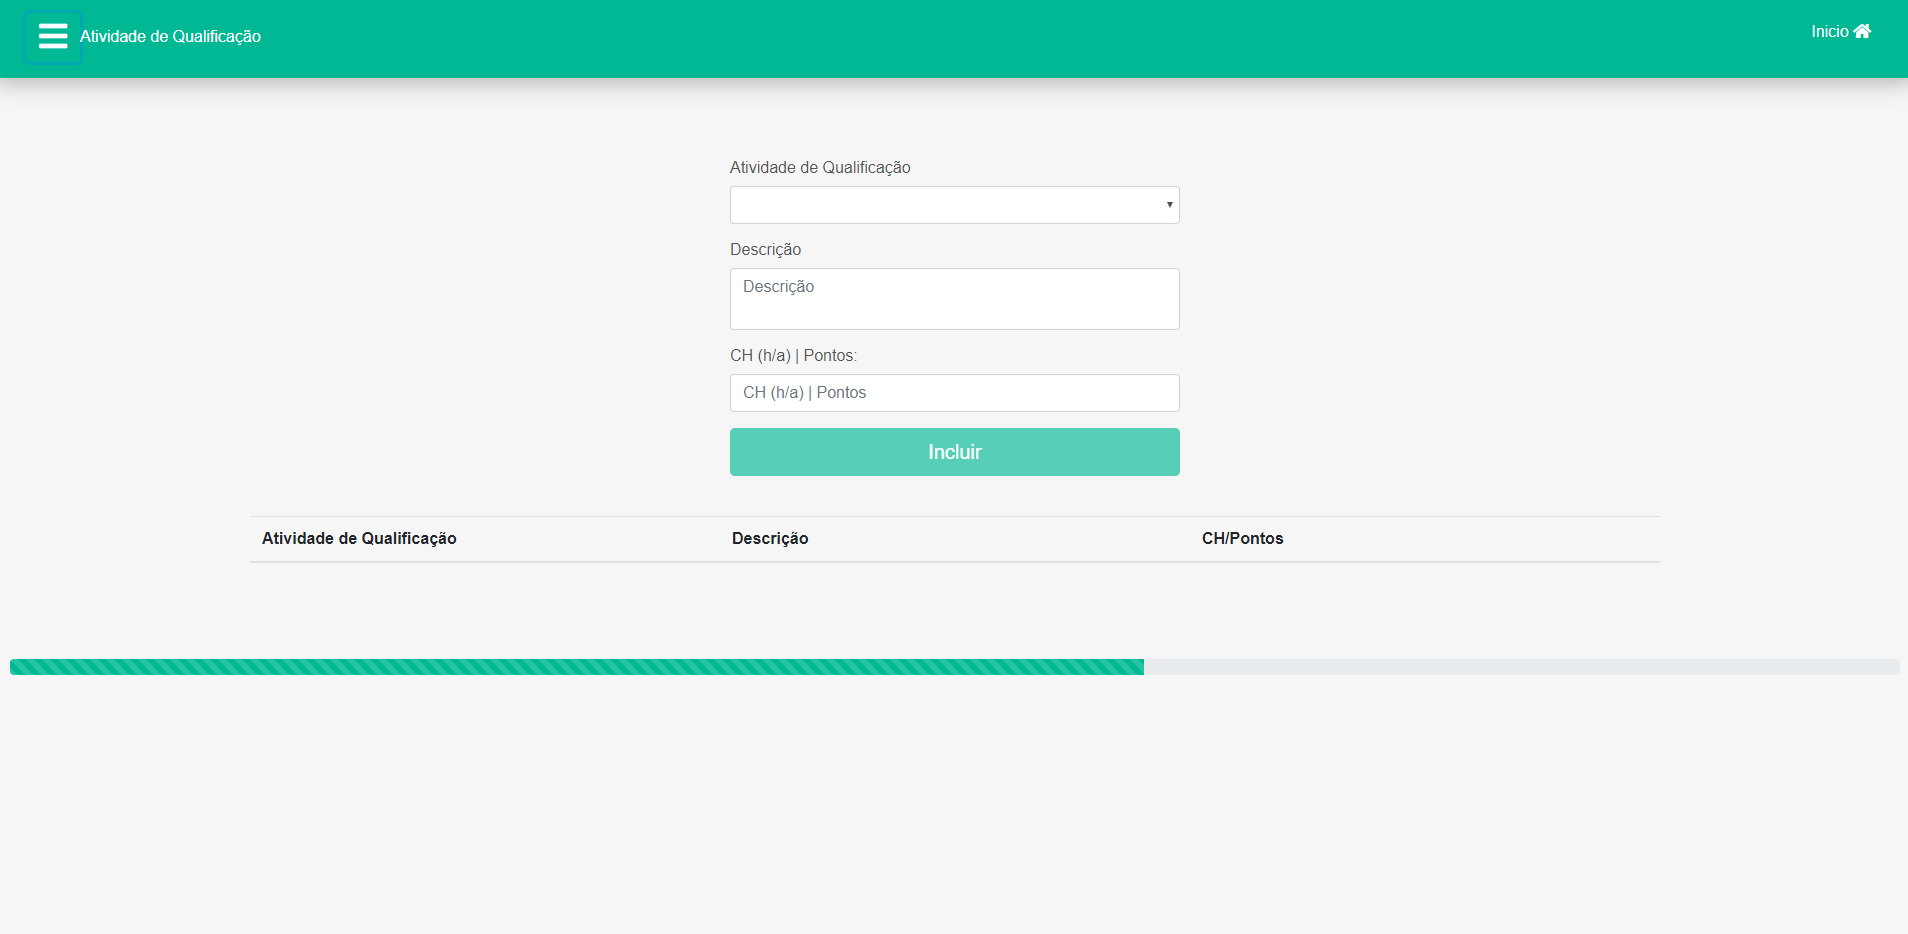
\includegraphics[width=.8\textwidth]{img/pagina_at_qualificacao.PNG}
    \caption[Resultado 08: Tela de Atividades Qualificação]{Resultado 08: Tela de Atividades Qualificação.}
    \label{fig:result08}
\end{figure}

\begin{figure}[htb]
    \centering
    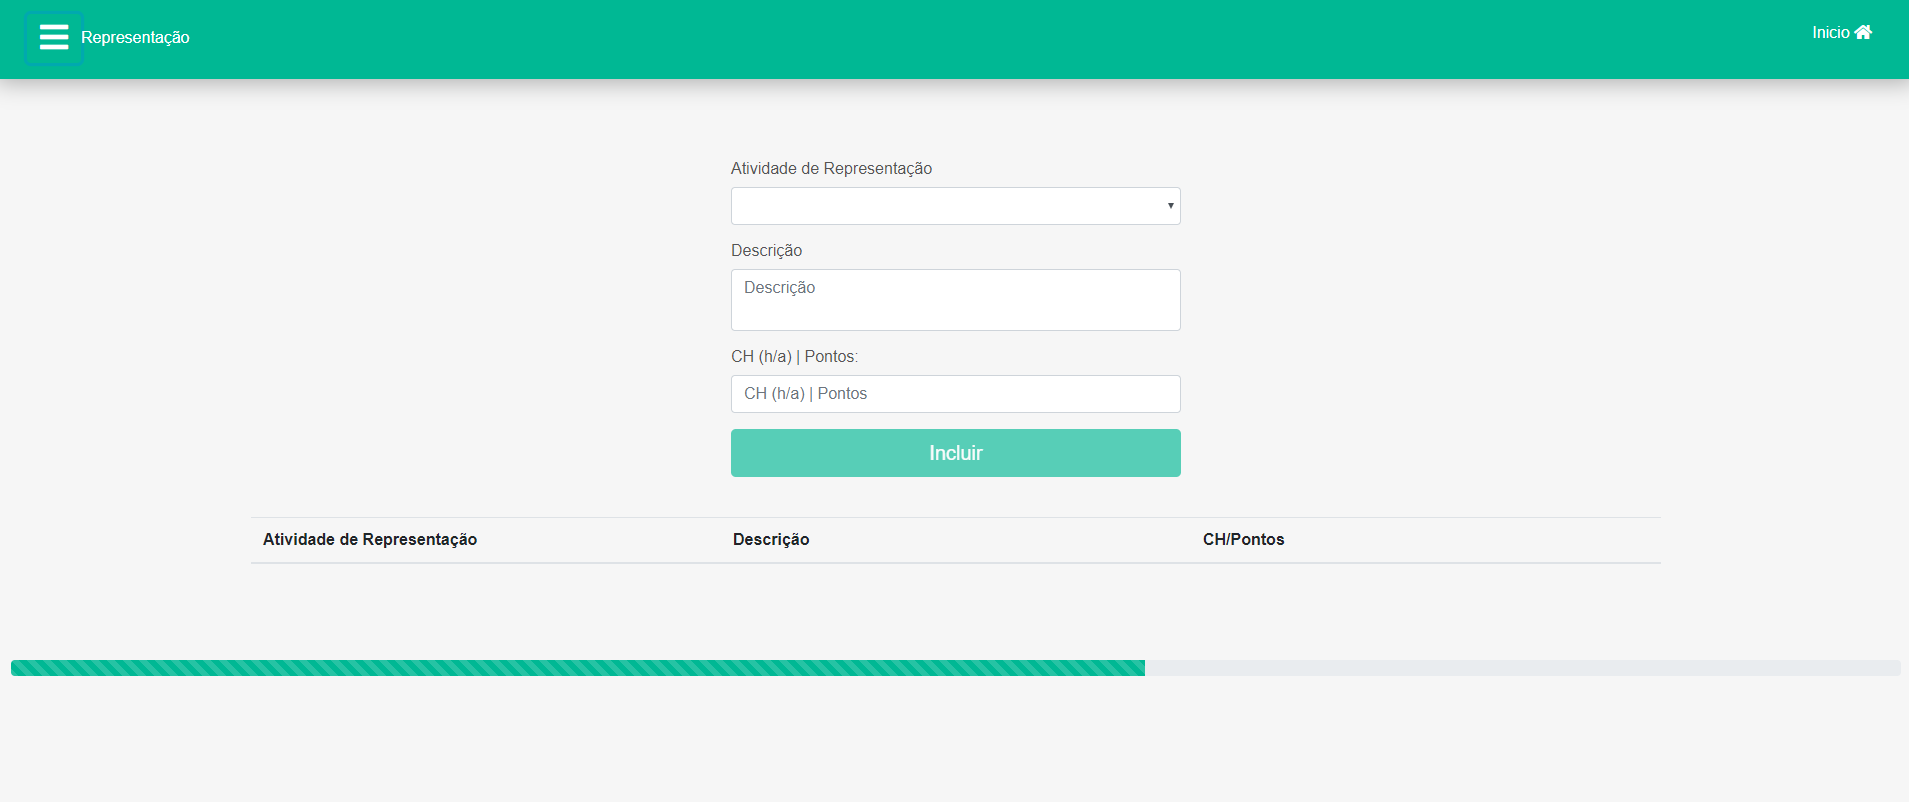
\includegraphics[width=.8\textwidth]{img/pagina_representacao.PNG}
    \caption[Resultado 09: Tela de Atividades Representação]{Resultado 09: Tela de Atividades Representação.}
    \label{fig:result09}
\end{figure}

\begin{figure}[htb]
    \centering
    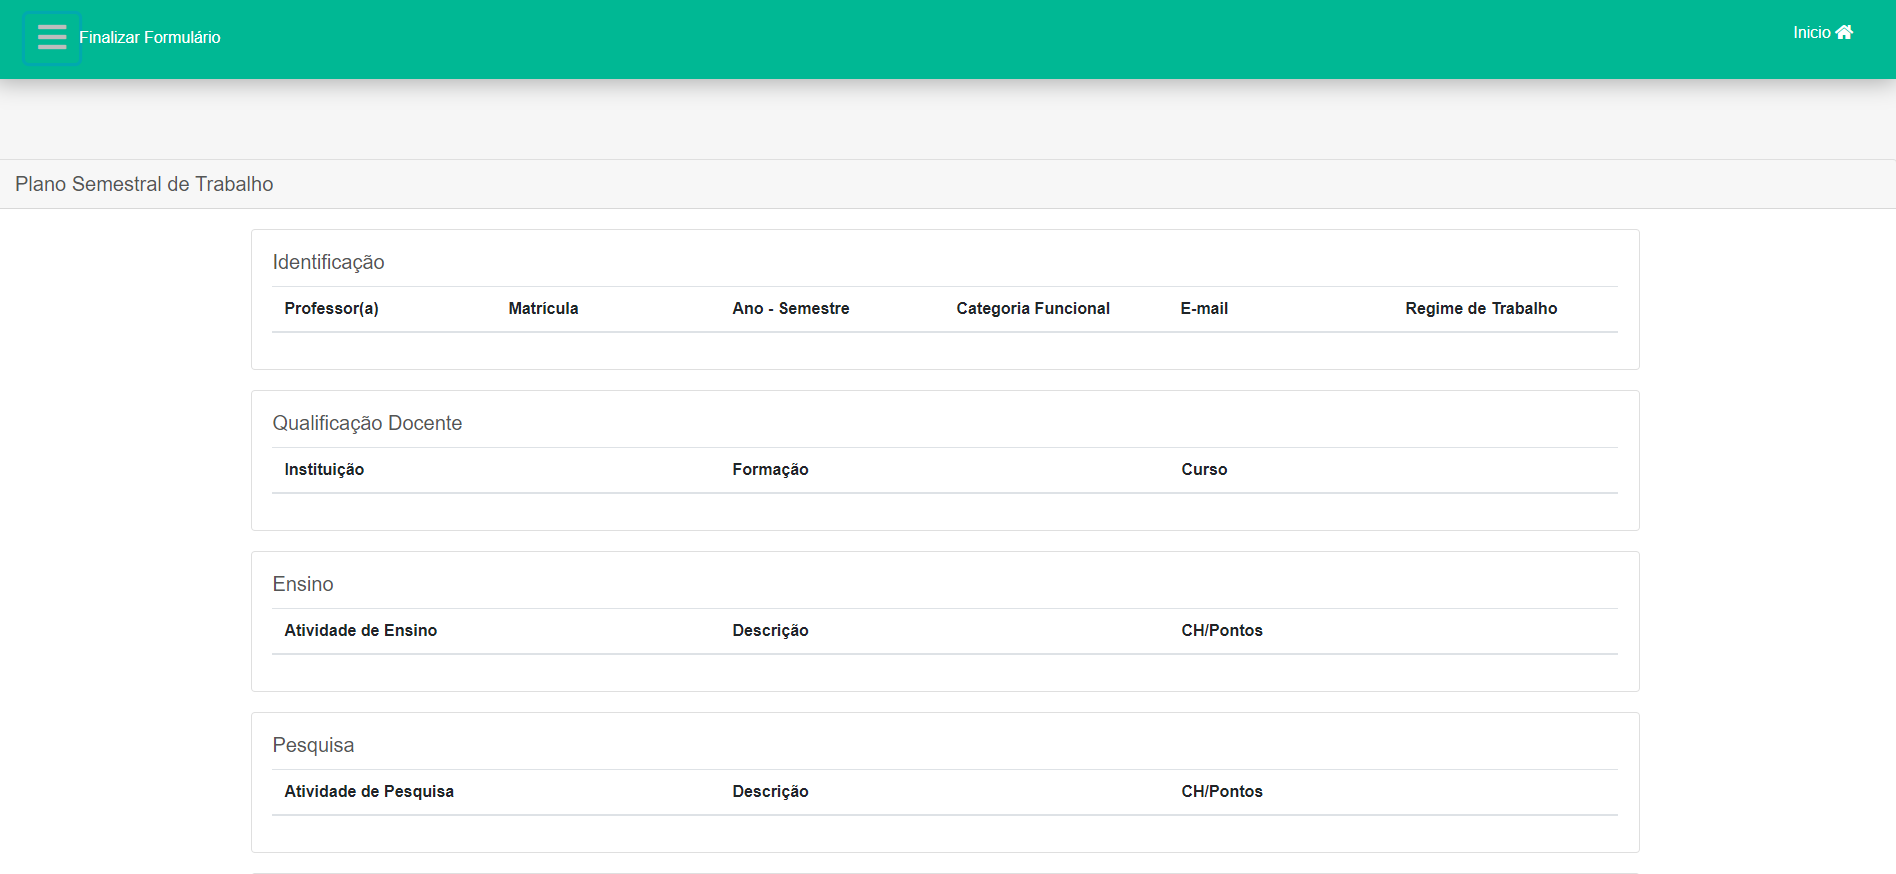
\includegraphics[width=.8\textwidth]{img/pagina_finalizar.PNG}
    \caption[Resultado 10: Tela de Finalização do Formulário]{Resultado 10: Tela de Finalização do Formulário.}
    \label{fig:result10}
\end{figure}

\begin{figure}[htb]
    \centering
    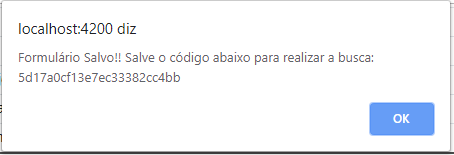
\includegraphics[width=.8\textwidth]{img/alert_salvar.PNG}
    \caption[Resultado 11: Tela de Mensagem de Formulário Salvo]{Resultado 11: Tela de Mensagem de Formulário Salvo.}
    \label{fig:result11}
\end{figure}

\begin{figure}[htb]
    \centering
    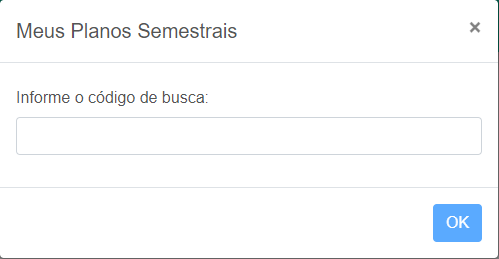
\includegraphics[width=.8\textwidth]{img/pagina_busca.PNG}
    \caption[Resultado 12: Tela de Busca do Formulário Salvo]{Resultado 12: Tela de Busca do Formulário Salvo.}
    \label{fig:result12}
\end{figure}

\chapter{Conclusão}
\label{Conclusao}


Foi desenvolvida uma primeira versão funcional (1.0) do sistema \textit{Web} \textit{e-Plano} para facilitar o preenchimento do Plano Semestral de Trabalho Docente, o qual é um instrumento de planejamento ao mesmo tempo para o docente e para a gestão do \acf{DAA} do \ac{IFG}.

Sendo um documento oficial auditável, é imperativo que o Plano Semestral de Trabalho Docente esteja coerente com a norma.
A aplicação garante ao docente e ao gestor, por meio da aplicação das \nameref{RegrasDeNegocio}, a conformidade do Plano Semestral de Trabalho Docente com a Resolução nº 9 do \ac{IFG}.

Utilizando tecnologias atuais do mercado de trabalho foi possível aplicar neste Trabalho de Conclusão de Curso uma variedade de conhecimentos adquirido ao longo do curso de Tecnologia em Análise e Desenvolvimento de Sistemas de forma integrada.
A experiência do desenvolvimento em uma situação de demanda real com prazos e recursos definidos foi fundamental para uma formação integral.

Melhorias planejadas da aplicação, incluem uma funcionalidade de envio de \textit{e-mail} para que o usuário receba o link de acesso ao formulário salvo, que pode ser visto na figura \ref{fig:prot10} de protótipo.
Além disso, é intenção o uso de um \textit{login} utilizando o serviço de autenticação do IFG via \textit{Web Service}, o qual depende da liberação por parte da Diretoria de Tecnologia da Informação.
Uma alternativa local para implantação está sendo construída usando o deploy via ``Docker container''~\footnote{http://dockerhub.com}.

\begin{figure}[htb]
    \centering
    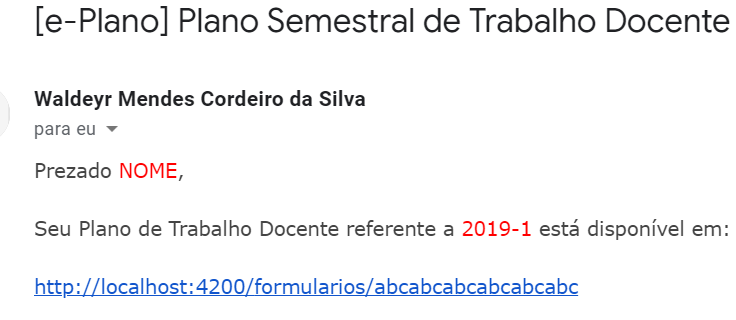
\includegraphics[width=0.5\textwidth]{img/email.PNG}
    \caption[Protótipo 10: \textit{E-mail}]{Protótipo 10: \textit{E-mail enviado pelo sistema para acesso ao Plano Semestral de Trabalho Docente}.}
    \label{fig:prot10}
\end{figure}

% References

\begin{references}
  \bibliography{bib/references}
\end{references}

% Appendix

%\theappendix
% %\chapter{Ata de Defesa do TCC}
\label{ap:ata}

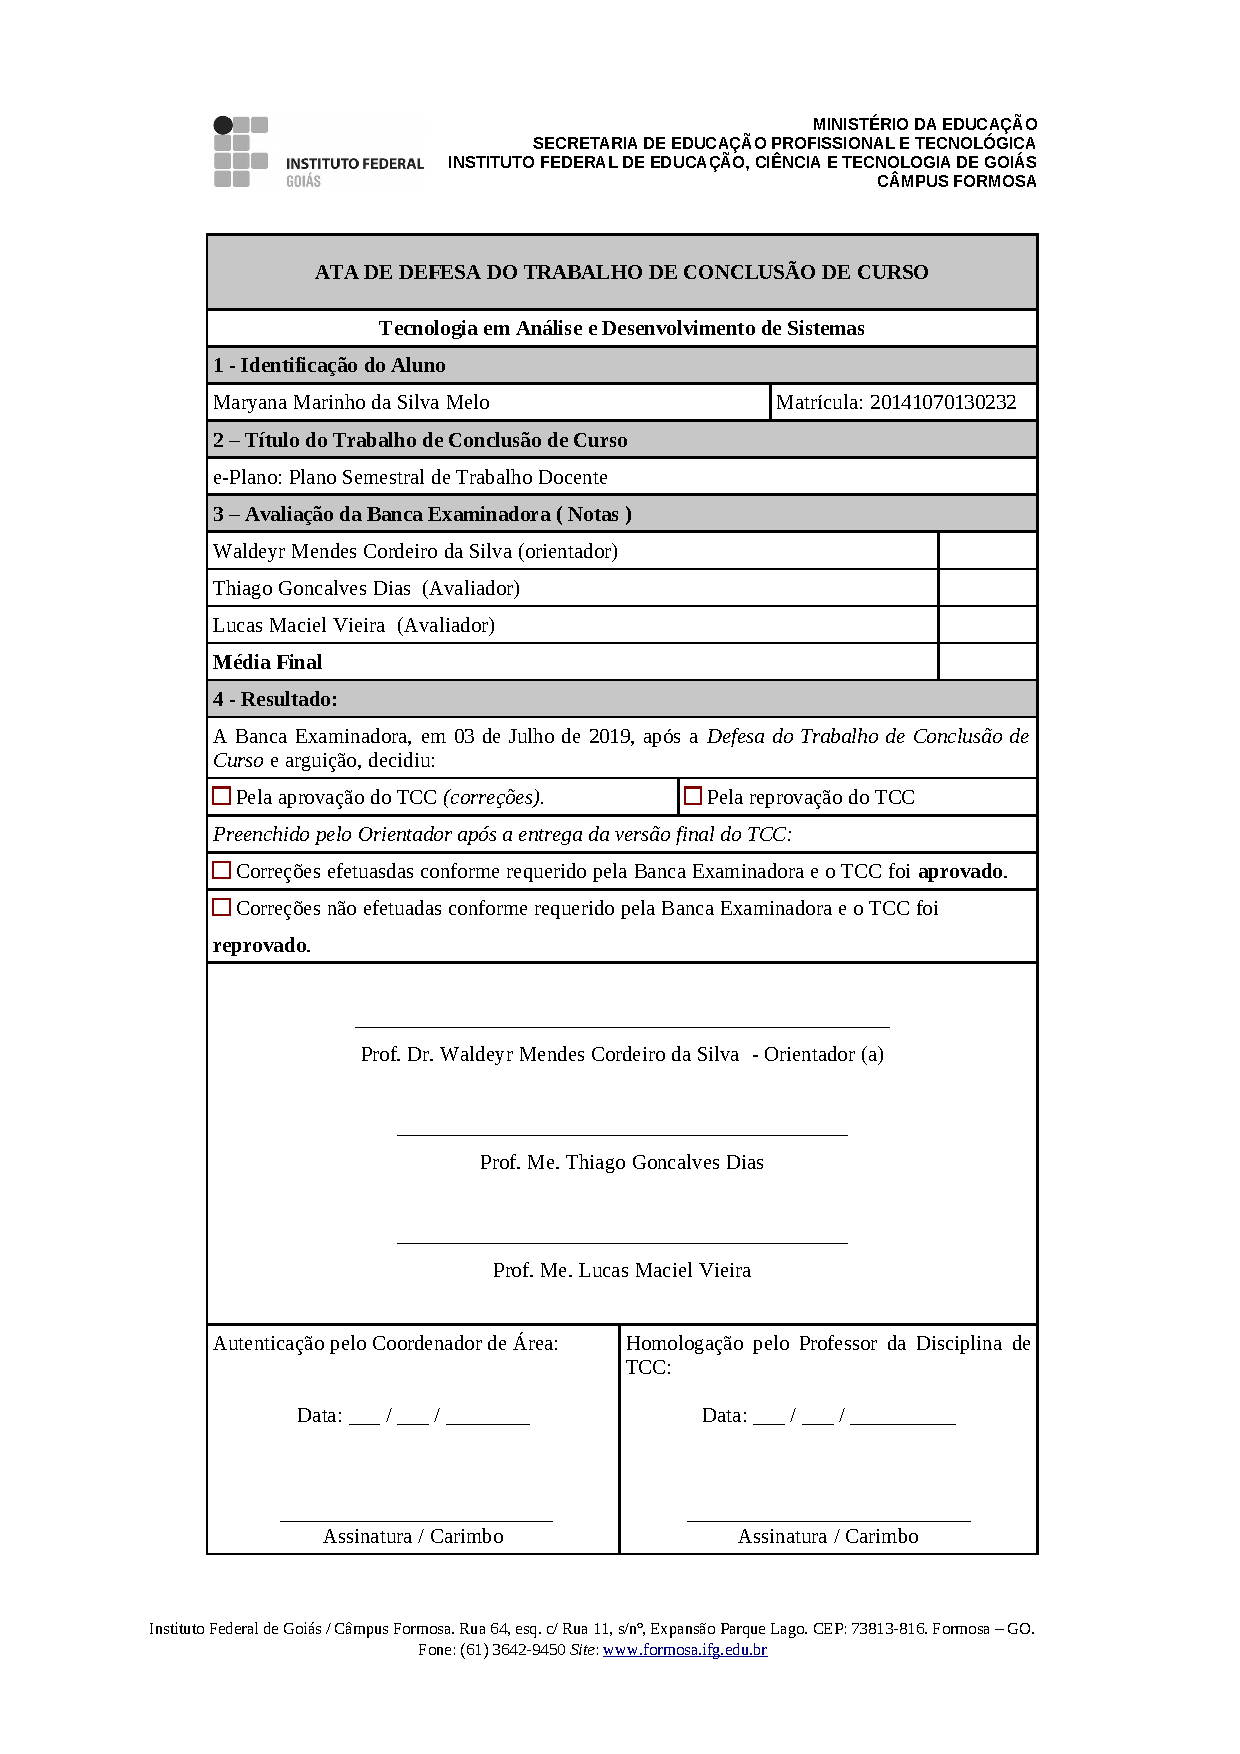
\includepdf[pages=-,offset=75 -75]{ModeloAta.pdf}



\end{document}
